\documentclass[twoside]{book}

% Packages required by doxygen
\usepackage{fixltx2e}
\usepackage{calc}
\usepackage{doxygen}
\usepackage[export]{adjustbox} % also loads graphicx
\usepackage{graphicx}
\usepackage[utf8]{inputenc}
\usepackage{makeidx}
\usepackage{multicol}
\usepackage{multirow}
\PassOptionsToPackage{warn}{textcomp}
\usepackage{textcomp}
\usepackage[nointegrals]{wasysym}
\usepackage[table]{xcolor}

% Font selection
\usepackage[T1]{fontenc}
\usepackage[scaled=.90]{helvet}
\usepackage{courier}
\usepackage{amssymb}
\usepackage{sectsty}
\renewcommand{\familydefault}{\sfdefault}
\allsectionsfont{%
  \fontseries{bc}\selectfont%
  \color{darkgray}%
}
\renewcommand{\DoxyLabelFont}{%
  \fontseries{bc}\selectfont%
  \color{darkgray}%
}
\newcommand{\+}{\discretionary{\mbox{\scriptsize$\hookleftarrow$}}{}{}}

% Page & text layout
\usepackage{geometry}
\geometry{%
  a4paper,%
  top=2.5cm,%
  bottom=2.5cm,%
  left=2.5cm,%
  right=2.5cm%
}
\tolerance=750
\hfuzz=15pt
\hbadness=750
\setlength{\emergencystretch}{15pt}
\setlength{\parindent}{0cm}
\setlength{\parskip}{3ex plus 2ex minus 2ex}
\makeatletter
\renewcommand{\paragraph}{%
  \@startsection{paragraph}{4}{0ex}{-1.0ex}{1.0ex}{%
    \normalfont\normalsize\bfseries\SS@parafont%
  }%
}
\renewcommand{\subparagraph}{%
  \@startsection{subparagraph}{5}{0ex}{-1.0ex}{1.0ex}{%
    \normalfont\normalsize\bfseries\SS@subparafont%
  }%
}
\makeatother

% Headers & footers
\usepackage{fancyhdr}
\pagestyle{fancyplain}
\fancyhead[LE]{\fancyplain{}{\bfseries\thepage}}
\fancyhead[CE]{\fancyplain{}{}}
\fancyhead[RE]{\fancyplain{}{\bfseries\leftmark}}
\fancyhead[LO]{\fancyplain{}{\bfseries\rightmark}}
\fancyhead[CO]{\fancyplain{}{}}
\fancyhead[RO]{\fancyplain{}{\bfseries\thepage}}
\fancyfoot[LE]{\fancyplain{}{}}
\fancyfoot[CE]{\fancyplain{}{}}
\fancyfoot[RE]{\fancyplain{}{\bfseries\scriptsize Generated by Doxygen }}
\fancyfoot[LO]{\fancyplain{}{\bfseries\scriptsize Generated by Doxygen }}
\fancyfoot[CO]{\fancyplain{}{}}
\fancyfoot[RO]{\fancyplain{}{}}
\renewcommand{\footrulewidth}{0.4pt}
\renewcommand{\chaptermark}[1]{%
  \markboth{#1}{}%
}
\renewcommand{\sectionmark}[1]{%
  \markright{\thesection\ #1}%
}

% Indices & bibliography
\usepackage{natbib}
\usepackage[titles]{tocloft}
\setcounter{tocdepth}{3}
\setcounter{secnumdepth}{5}
\makeindex

% Hyperlinks (required, but should be loaded last)
\usepackage{ifpdf}
\ifpdf
  \usepackage[pdftex,pagebackref=true]{hyperref}
\else
  \usepackage[ps2pdf,pagebackref=true]{hyperref}
\fi
\hypersetup{%
  colorlinks=true,%
  linkcolor=blue,%
  citecolor=blue,%
  unicode%
}

% Custom commands
\newcommand{\clearemptydoublepage}{%
  \newpage{\pagestyle{empty}\cleardoublepage}%
}

\usepackage{caption}
\captionsetup{labelsep=space,justification=centering,font={bf},singlelinecheck=off,skip=4pt,position=top}

%===== C O N T E N T S =====

\begin{document}

% Titlepage & ToC
\hypersetup{pageanchor=false,
             bookmarksnumbered=true,
             pdfencoding=unicode
            }
\pagenumbering{alph}
\begin{titlepage}
\vspace*{7cm}
\begin{center}%
{\Large Codice Sistemi Embedded }\\
\vspace*{1cm}
{\large Generated by Doxygen 1.8.13}\\
\end{center}
\end{titlepage}
\clearemptydoublepage
\pagenumbering{roman}
\tableofcontents
\clearemptydoublepage
\pagenumbering{arabic}
\hypersetup{pageanchor=true}

%--- Begin generated contents ---
\chapter{Documentazione codice sistemi embedded}
\label{index}\hypertarget{index}{}\begin{DoxyParagraph}{Table of Contents}

\end{DoxyParagraph}
\hypertarget{index_GPIO}{}\section{G\+P\+IO}\label{index_GPIO}
\hypertarget{index_Driver}{}\subsection{Driver}\label{index_Driver}

\begin{DoxyItemize}
\item Funzioni driver G\+P\+IO \hyperlink{gpio__int_8c}{gpio\+\_\+int.\+c} 
\end{DoxyItemize}\hypertarget{index_Hardware}{}\subsection{Hardware}\label{index_Hardware}

\begin{DoxyItemize}
\item Controlla la generazione dell\textquotesingle{} interrupt \hyperlink{GPIO__v1__0__S00__AXI_8vhd}{G\+P\+I\+O\+\_\+v1\+\_\+0\+\_\+\+S00\+\_\+\+A\+X\+I.\+vhd}
\item Top level entity del componente \hyperlink{classGPIO__v1__0__S00__AXI}{G\+P\+I\+O\+\_\+v1\+\_\+0\+\_\+\+S00\+\_\+\+A\+XI} \hyperlink{GPIO__v1__0_8vhd}{G\+P\+I\+O\+\_\+v1\+\_\+0.\+vhd} 
\end{DoxyItemize}\hypertarget{index_UART}{}\section{U\+A\+RT}\label{index_UART}
\hypertarget{index_Driver}{}\subsection{Driver}\label{index_Driver}
\hypertarget{index_UIO}{}\subsubsection{U\+IO}\label{index_UIO}

\begin{DoxyItemize}
\item gestione del componente U\+A\+RT utilizzando il driver uio U\+A\+R\+T\+\_\+interrupt\+\_\+uio.\+c 
\end{DoxyItemize}\hypertarget{index_KERNEL}{}\subsubsection{K\+E\+R\+N\+EL}\label{index_KERNEL}

\begin{DoxyItemize}
\item gestione del componente U\+A\+RT in modalità kernel \hyperlink{UART__interrupt__kernel__mode_8c}{U\+A\+R\+T\+\_\+interrupt\+\_\+kernel\+\_\+mode.\+c} 
\end{DoxyItemize}\hypertarget{index_Hardware}{}\subsection{Hardware}\label{index_Hardware}

\begin{DoxyItemize}
\item Controlla la generazione dell\textquotesingle{} interrupt \hyperlink{UART__v1__0__S00__AXI_8vhd}{U\+A\+R\+T\+\_\+v1\+\_\+0\+\_\+\+S00\+\_\+\+A\+X\+I.\+vhd}
\item Top level entity del componente \hyperlink{classUART__v1__0__S00__AXI}{U\+A\+R\+T\+\_\+v1\+\_\+0\+\_\+\+S00\+\_\+\+A\+XI} \hyperlink{UART__v1__0_8vhd}{U\+A\+R\+T\+\_\+v1\+\_\+0.\+vhd} 
\end{DoxyItemize}\hypertarget{index_CRC}{}\section{C\+RC}\label{index_CRC}
@ F3
\begin{DoxyItemize}
\item gestione dell\textquotesingle{} invio, calcolo e check del C\+RC \hyperlink{STM32_2CRC__Revisited__loop_2src_2main_8c}{main.\+c} 
\end{DoxyItemize}
\chapter{driver\+\_\+\+G\+P\+IO}
\label{driver_GPIO}
\Hypertarget{driver_GPIO}
Funzioni per l\textquotesingle{}utilizzo della periferiferica \hyperlink{structGPIO}{G\+P\+IO} 
\chapter{Design Unit Index}
\section{Design Unit Hierarchy}
This inheritance list is sorted roughly, but not completely, alphabetically\+:\begin{DoxyCompactList}
\item \contentsline{section}{G\+P\+IO}{\pageref{structGPIO}}{}
\item \contentsline{section}{G\+P\+I\+O\+\_\+list}{\pageref{structGPIO__list}}{}
\item \contentsline{section}{G\+P\+I\+O\+\_\+v1\+\_\+0}{\pageref{classGPIO__v1__0}}{}
\begin{DoxyCompactList}
\item \contentsline{section}{G\+P\+I\+O\+\_\+v1\+\_\+0\+\_\+\+S00\+\_\+\+A\+XI}{\pageref{classGPIO__v1__0__S00__AXI}}{}
\end{DoxyCompactList}
\item \contentsline{section}{U\+A\+R\+T\+\_\+v1\+\_\+0}{\pageref{classUART__v1__0}}{}
\begin{DoxyCompactList}
\item \contentsline{section}{U\+A\+R\+T\+\_\+v1\+\_\+0\+\_\+\+S00\+\_\+\+A\+XI}{\pageref{classUART__v1__0__S00__AXI}}{}
\end{DoxyCompactList}
\end{DoxyCompactList}

\chapter{Design Unit Index}
\section{Design Unit List}
Here is a list of all design unit members with links to the Entities they belong to\+:\begin{DoxyCompactList}
\item\contentsline{section}{architecture \hyperlink{classGPIO__v1__0_1_1arch__imp}{arch\+\_\+imp} }{\pageref{classGPIO__v1__0_1_1arch__imp}}{}
\item\contentsline{section}{architecture \hyperlink{classGPIO__v1__0__S00__AXI_1_1arch__imp}{arch\+\_\+imp} }{\pageref{classGPIO__v1__0__S00__AXI_1_1arch__imp}}{}
\item\contentsline{section}{architecture \hyperlink{classUART__v1__0__S00__AXI_1_1arch__imp}{arch\+\_\+imp} }{\pageref{classUART__v1__0__S00__AXI_1_1arch__imp}}{}
\item\contentsline{section}{architecture \hyperlink{classUART__v1__0_1_1arch__imp}{arch\+\_\+imp} \\*Componente U\+A\+R\+T\+\_\+\+A\+X\+I\+\_\+\+S00  componente nel quale è incapsulato il componente U\+A\+RT e la logica di gestione delle interruzioni }{\pageref{classUART__v1__0_1_1arch__imp}}{}
\item\contentsline{section}{entity \hyperlink{classGPIO__v1__0}{G\+P\+I\+O\+\_\+v1\+\_\+0} }{\pageref{classGPIO__v1__0}}{}
\item\contentsline{section}{entity \hyperlink{classGPIO__v1__0__S00__AXI}{G\+P\+I\+O\+\_\+v1\+\_\+0\+\_\+\+S00\+\_\+\+A\+XI} }{\pageref{classGPIO__v1__0__S00__AXI}}{}
\item\contentsline{section}{\hyperlink{structmydriver__dm}{mydriver\+\_\+dm} }{\pageref{structmydriver__dm}}{}
\item\contentsline{section}{\hyperlink{structmyIntGPIO}{my\+Int\+G\+P\+IO} }{\pageref{structmyIntGPIO}}{}
\item\contentsline{section}{entity \hyperlink{classUART__v1__0}{U\+A\+R\+T\+\_\+v1\+\_\+0} }{\pageref{classUART__v1__0}}{}
\item\contentsline{section}{entity \hyperlink{classUART__v1__0__S00__AXI}{U\+A\+R\+T\+\_\+v1\+\_\+0\+\_\+\+S00\+\_\+\+A\+XI} }{\pageref{classUART__v1__0__S00__AXI}}{}
\end{DoxyCompactList}

\chapter{File Index}
\section{File List}
Here is a list of all documented files with brief descriptions\+:\begin{DoxyCompactList}
\item\contentsline{section}{/media/saverio/\+O\+S/\+Users/\+Saverio/\+Desktop/\+S\+E/git/\+Andrea/\+F\+P\+G\+A/\+G\+P\+I\+O\+With\+Interrupt/\+G\+P\+I\+O\+With\+Interrupt.\+sdk/\+G\+P\+I\+O/src/\hyperlink{gpio__int_8c}{gpio\+\_\+int.\+c} }{\pageref{gpio__int_8c}}{}
\item\contentsline{section}{/media/saverio/\+O\+S/\+Users/\+Saverio/\+Desktop/\+S\+E/git/\+Andrea/\+F\+P\+G\+A/\+G\+P\+I\+O\+With\+Interrupt/\+G\+P\+I\+O\+With\+Interrupt.\+sdk/\+G\+P\+I\+O/src/{\bfseries gpio\+\_\+int.\+h} }{\pageref{gpio__int_8h}}{}
\item\contentsline{section}{/media/saverio/\+O\+S/\+Users/\+Saverio/\+Desktop/\+S\+E/git/\+Andrea/\+F\+P\+G\+A/ip\+\_\+repo/\+G\+P\+I\+O\+\_\+1.\+0/hdl/\hyperlink{GPIO__v1__0_8vhd}{G\+P\+I\+O\+\_\+v1\+\_\+0.\+vhd} \\*Top level entity del custom IP core G\+P\+I\+O\+\_\+\+V1\+\_\+0\+\_\+\+S00\+\_\+\+A\+X\+I.\+V\+HD }{\pageref{GPIO__v1__0_8vhd}}{}
\item\contentsline{section}{/media/saverio/\+O\+S/\+Users/\+Saverio/\+Desktop/\+S\+E/git/\+Andrea/\+F\+P\+G\+A/ip\+\_\+repo/\+G\+P\+I\+O\+\_\+1.\+0/hdl/\hyperlink{GPIO__v1__0__S00__AXI_8vhd}{G\+P\+I\+O\+\_\+v1\+\_\+0\+\_\+\+S00\+\_\+\+A\+X\+I.\+vhd} \\*Componente utilizzato collegare il G\+P\+IO al bus A\+XI e gestire le interruzioni }{\pageref{GPIO__v1__0__S00__AXI_8vhd}}{}
\item\contentsline{section}{/media/saverio/\+O\+S/\+Users/\+Saverio/\+Desktop/\+S\+E/git/\+Andrea/\+F\+P\+G\+A/ip\+\_\+repo/\+U\+A\+R\+T\+\_\+1.\+0/hdl/\hyperlink{UART__v1__0_8vhd}{U\+A\+R\+T\+\_\+v1\+\_\+0.\+vhd} \\*U\+A\+RT A\+XI I\+P\+C\+O\+RE with interrupt }{\pageref{UART__v1__0_8vhd}}{}
\item\contentsline{section}{/media/saverio/\+O\+S/\+Users/\+Saverio/\+Desktop/\+S\+E/git/\+Andrea/\+F\+P\+G\+A/ip\+\_\+repo/\+U\+A\+R\+T\+\_\+1.\+0/hdl/\hyperlink{UART__v1__0__S00__AXI_8vhd}{U\+A\+R\+T\+\_\+v1\+\_\+0\+\_\+\+S00\+\_\+\+A\+X\+I.\+vhd} \\*U\+A\+RT A\+XI I\+P\+C\+O\+RE with interrupt }{\pageref{UART__v1__0__S00__AXI_8vhd}}{}
\end{DoxyCompactList}

\chapter{Data Structure Documentation}
\hypertarget{classGPIO__v1__0_1_1arch__imp}{}\section{arch\+\_\+imp Architecture Reference}
\label{classGPIO__v1__0_1_1arch__imp}\index{arch\+\_\+imp@{arch\+\_\+imp}}
\subsection*{Components}
 \begin{DoxyCompactItemize}
\item 
\mbox{\Hypertarget{classGPIO__v1__0_1_1arch__imp_acfa88fcc633c72af8bfd7e652932f7c7}\label{classGPIO__v1__0_1_1arch__imp_acfa88fcc633c72af8bfd7e652932f7c7}} 
\hyperlink{classGPIO__v1__0_1_1arch__imp_acfa88fcc633c72af8bfd7e652932f7c7}{G\+P\+I\+O\+\_\+v1\+\_\+0\+\_\+\+S00\+\_\+\+A\+XI}  {\bfseries }  
\end{DoxyCompactItemize}
\subsection*{Instantiations}
 \begin{DoxyCompactItemize}
\item 
\mbox{\Hypertarget{classGPIO__v1__0_1_1arch__imp_add7a292f6a3530426561c0d1bf9540b4}\label{classGPIO__v1__0_1_1arch__imp_add7a292f6a3530426561c0d1bf9540b4}} 
\hyperlink{classGPIO__v1__0_1_1arch__imp_add7a292f6a3530426561c0d1bf9540b4}{gpio\+\_\+v1\+\_\+0\+\_\+s00\+\_\+axi\+\_\+inst}  {\bfseries G\+P\+I\+O\+\_\+v1\+\_\+0\+\_\+\+S00\+\_\+\+A\+XI}   
\end{DoxyCompactItemize}


The documentation for this class was generated from the following file\+:\begin{DoxyCompactItemize}
\item 
/media/saverio/\+O\+S/\+Users/\+Saverio/\+Desktop/\+S\+E/git/\+Andrea/\+F\+P\+G\+A/ip\+\_\+repo/\+G\+P\+I\+O\+\_\+1.\+0/hdl/\hyperlink{GPIO__v1__0_8vhd}{G\+P\+I\+O\+\_\+v1\+\_\+0.\+vhd}\end{DoxyCompactItemize}

\hypertarget{classGPIO__v1__0__S00__AXI_1_1arch__imp}{}\section{arch\+\_\+imp Architecture Reference}
\label{classGPIO__v1__0__S00__AXI_1_1arch__imp}\index{arch\+\_\+imp@{arch\+\_\+imp}}
\subsection*{Processes}
 \begin{DoxyCompactItemize}
\item 
\mbox{\Hypertarget{classGPIO__v1__0__S00__AXI_1_1arch__imp_a655ff15956b68ed88b52a952f269c553}\label{classGPIO__v1__0__S00__AXI_1_1arch__imp_a655ff15956b68ed88b52a952f269c553}} 
\hyperlink{classGPIO__v1__0__S00__AXI_1_1arch__imp_a655ff15956b68ed88b52a952f269c553}{P\+R\+O\+C\+E\+S\+S\+\_\+0}{\bfseries  ( {\bfseries \textcolor{vhdlchar}{S\+\_\+\+A\+X\+I\+\_\+\+A\+C\+LK}\textcolor{vhdlchar}{ }} )}
\item 
\mbox{\Hypertarget{classGPIO__v1__0__S00__AXI_1_1arch__imp_a973f7a24b3f37478f610ab542f0e5086}\label{classGPIO__v1__0__S00__AXI_1_1arch__imp_a973f7a24b3f37478f610ab542f0e5086}} 
\hyperlink{classGPIO__v1__0__S00__AXI_1_1arch__imp_a973f7a24b3f37478f610ab542f0e5086}{P\+R\+O\+C\+E\+S\+S\+\_\+1}{\bfseries  ( {\bfseries \textcolor{vhdlchar}{S\+\_\+\+A\+X\+I\+\_\+\+A\+C\+LK}\textcolor{vhdlchar}{ }} )}
\item 
\mbox{\Hypertarget{classGPIO__v1__0__S00__AXI_1_1arch__imp_a5625666cb3140d01797433f2f6d93982}\label{classGPIO__v1__0__S00__AXI_1_1arch__imp_a5625666cb3140d01797433f2f6d93982}} 
\hyperlink{classGPIO__v1__0__S00__AXI_1_1arch__imp_a5625666cb3140d01797433f2f6d93982}{P\+R\+O\+C\+E\+S\+S\+\_\+2}{\bfseries  ( {\bfseries \textcolor{vhdlchar}{S\+\_\+\+A\+X\+I\+\_\+\+A\+C\+LK}\textcolor{vhdlchar}{ }} )}
\item 
\mbox{\Hypertarget{classGPIO__v1__0__S00__AXI_1_1arch__imp_a4bfd183cdd84fed1accdc6dcabc8fc3c}\label{classGPIO__v1__0__S00__AXI_1_1arch__imp_a4bfd183cdd84fed1accdc6dcabc8fc3c}} 
\hyperlink{classGPIO__v1__0__S00__AXI_1_1arch__imp_a4bfd183cdd84fed1accdc6dcabc8fc3c}{P\+R\+O\+C\+E\+S\+S\+\_\+3}{\bfseries  ( {\bfseries \textcolor{vhdlchar}{S\+\_\+\+A\+X\+I\+\_\+\+A\+C\+LK}\textcolor{vhdlchar}{ }} )}
\item 
\mbox{\Hypertarget{classGPIO__v1__0__S00__AXI_1_1arch__imp_a78c6c876515e14c79fe38dcb286ce0f1}\label{classGPIO__v1__0__S00__AXI_1_1arch__imp_a78c6c876515e14c79fe38dcb286ce0f1}} 
\hyperlink{classGPIO__v1__0__S00__AXI_1_1arch__imp_a78c6c876515e14c79fe38dcb286ce0f1}{P\+R\+O\+C\+E\+S\+S\+\_\+4}{\bfseries  ( {\bfseries \textcolor{vhdlchar}{S\+\_\+\+A\+X\+I\+\_\+\+A\+C\+LK}\textcolor{vhdlchar}{ }} )}
\item 
\mbox{\Hypertarget{classGPIO__v1__0__S00__AXI_1_1arch__imp_aeef87657fc8d27430790f1e6088ab81f}\label{classGPIO__v1__0__S00__AXI_1_1arch__imp_aeef87657fc8d27430790f1e6088ab81f}} 
\hyperlink{classGPIO__v1__0__S00__AXI_1_1arch__imp_aeef87657fc8d27430790f1e6088ab81f}{P\+R\+O\+C\+E\+S\+S\+\_\+5}{\bfseries  ( {\bfseries \textcolor{vhdlchar}{S\+\_\+\+A\+X\+I\+\_\+\+A\+C\+LK}\textcolor{vhdlchar}{ }} )}
\item 
\mbox{\Hypertarget{classGPIO__v1__0__S00__AXI_1_1arch__imp_a7390c9b34974c278e7646b784061d076}\label{classGPIO__v1__0__S00__AXI_1_1arch__imp_a7390c9b34974c278e7646b784061d076}} 
\hyperlink{classGPIO__v1__0__S00__AXI_1_1arch__imp_a7390c9b34974c278e7646b784061d076}{P\+R\+O\+C\+E\+S\+S\+\_\+6}{\bfseries  ( {\bfseries \textcolor{vhdlchar}{S\+\_\+\+A\+X\+I\+\_\+\+A\+C\+LK}\textcolor{vhdlchar}{ }} )}
\item 
\mbox{\Hypertarget{classGPIO__v1__0__S00__AXI_1_1arch__imp_a7eca128197092fa81fcaaba67313360f}\label{classGPIO__v1__0__S00__AXI_1_1arch__imp_a7eca128197092fa81fcaaba67313360f}} 
\hyperlink{classGPIO__v1__0__S00__AXI_1_1arch__imp_a7eca128197092fa81fcaaba67313360f}{P\+R\+O\+C\+E\+S\+S\+\_\+7}{\bfseries  ( {\bfseries \textcolor{vhdlchar}{slv\+\_\+reg0}\textcolor{vhdlchar}{ }} , {\bfseries \textcolor{vhdlchar}{slv\+\_\+reg1}\textcolor{vhdlchar}{ }} , {\bfseries \textcolor{vhdlchar}{gpio\+\_\+read}\textcolor{vhdlchar}{ }} , {\bfseries \textcolor{vhdlchar}{slv\+\_\+reg3}\textcolor{vhdlchar}{ }} , {\bfseries \textcolor{vhdlchar}{slv\+\_\+reg4}\textcolor{vhdlchar}{ }} , {\bfseries \textcolor{vhdlchar}{slv\+\_\+reg5}\textcolor{vhdlchar}{ }} , {\bfseries \textcolor{vhdlchar}{status\+\_\+reg\+\_\+out}\textcolor{vhdlchar}{ }} , {\bfseries \textcolor{vhdlchar}{slv\+\_\+reg7\+\_\+out}\textcolor{vhdlchar}{ }} , {\bfseries \textcolor{vhdlchar}{axi\+\_\+araddr}\textcolor{vhdlchar}{ }} , {\bfseries \textcolor{vhdlchar}{S\+\_\+\+A\+X\+I\+\_\+\+A\+R\+E\+S\+E\+TN}\textcolor{vhdlchar}{ }} , {\bfseries \textcolor{vhdlchar}{slv\+\_\+reg\+\_\+rden}\textcolor{vhdlchar}{ }} )}
\item 
\mbox{\Hypertarget{classGPIO__v1__0__S00__AXI_1_1arch__imp_a45eef1701e94703c5a3cf169c02e5e2c}\label{classGPIO__v1__0__S00__AXI_1_1arch__imp_a45eef1701e94703c5a3cf169c02e5e2c}} 
\hyperlink{classGPIO__v1__0__S00__AXI_1_1arch__imp_a45eef1701e94703c5a3cf169c02e5e2c}{P\+R\+O\+C\+E\+S\+S\+\_\+8}{\bfseries  ( {\bfseries \textcolor{vhdlchar}{S\+\_\+\+A\+X\+I\+\_\+\+A\+C\+LK}\textcolor{vhdlchar}{ }} )}
\item 
\hyperlink{classGPIO__v1__0__S00__AXI_1_1arch__imp_a29a70265aec87dff63669cc686cdd7b6}{gpio\+\_\+read\+\_\+sampling}{\bfseries  ( {\bfseries \textcolor{vhdlchar}{S\+\_\+\+A\+X\+I\+\_\+\+A\+C\+LK}\textcolor{vhdlchar}{ }} , {\bfseries \textcolor{vhdlchar}{gpio\+\_\+read}\textcolor{vhdlchar}{ }} )}
\begin{DoxyCompactList}\small\item\em Campiona i segnali di cui si vuole verificare la generazione di un interrupt. \end{DoxyCompactList}\item 
\hyperlink{classGPIO__v1__0__S00__AXI_1_1arch__imp_a27a13ac4e8c3307360aa906035c2e140}{intr\+\_\+pending}{\bfseries  ( {\bfseries \textcolor{vhdlchar}{S\+\_\+\+A\+X\+I\+\_\+\+A\+C\+LK}\textcolor{vhdlchar}{ }} , {\bfseries \textcolor{vhdlchar}{change\+\_\+detected}\textcolor{vhdlchar}{ }} , {\bfseries \textcolor{vhdlchar}{ack\+\_\+intr}\textcolor{vhdlchar}{ }} , {\bfseries \textcolor{vhdlchar}{pending\+\_\+intr\+\_\+tmp}\textcolor{vhdlchar}{ }} )}
\begin{DoxyCompactList}\small\item\em Gestisce il registro pending. \end{DoxyCompactList}\item 
\hyperlink{classGPIO__v1__0__S00__AXI_1_1arch__imp_ad49f0dfc577739899b90a7243c22a1cd}{inst\+\_\+irq}{\bfseries  ( {\bfseries \textcolor{vhdlchar}{S\+\_\+\+A\+X\+I\+\_\+\+A\+C\+LK}\textcolor{vhdlchar}{ }} , {\bfseries \textcolor{vhdlchar}{pending\+\_\+intr}\textcolor{vhdlchar}{ }} , {\bfseries \textcolor{vhdlchar}{global\+\_\+intr}\textcolor{vhdlchar}{ }} )}
\begin{DoxyCompactList}\small\item\em Disabilita l\textquotesingle{} interrupt nel caso di reset del bus e tiene alto il segnale di interrupt finchè rimane pendente. \end{DoxyCompactList}\end{DoxyCompactItemize}
\subsection*{Components}
 \begin{DoxyCompactItemize}
\item 
\mbox{\Hypertarget{classGPIO__v1__0__S00__AXI_1_1arch__imp_a7f7f55a1fb49e8857e13928560e7c192}\label{classGPIO__v1__0__S00__AXI_1_1arch__imp_a7f7f55a1fb49e8857e13928560e7c192}} 
\hyperlink{classGPIO__v1__0__S00__AXI_1_1arch__imp_a7f7f55a1fb49e8857e13928560e7c192}{G\+P\+I\+O\+\_\+\+Array}  {\bfseries }  
\end{DoxyCompactItemize}
\subsection*{Constants}
 \begin{DoxyCompactItemize}
\item 
\mbox{\Hypertarget{classGPIO__v1__0__S00__AXI_1_1arch__imp_a92f00d1b43f901f1bf5684d1e79aab84}\label{classGPIO__v1__0__S00__AXI_1_1arch__imp_a92f00d1b43f901f1bf5684d1e79aab84}} 
\hyperlink{classGPIO__v1__0__S00__AXI_1_1arch__imp_a92f00d1b43f901f1bf5684d1e79aab84}{A\+D\+D\+R\+\_\+\+L\+SB} {\bfseries \textcolor{vhdlchar}{integer}\textcolor{vhdlchar}{ }\textcolor{vhdlchar}{ }\textcolor{vhdlchar}{\+:}\textcolor{vhdlchar}{=}\textcolor{vhdlchar}{ }\textcolor{vhdlchar}{(}\textcolor{vhdlchar}{ }\textcolor{vhdlchar}{ }\textcolor{vhdlchar}{ }\textcolor{vhdlchar}{ }\textcolor{vhdlchar}{C\+\_\+\+S\+\_\+\+A\+X\+I\+\_\+\+D\+A\+T\+A\+\_\+\+W\+I\+D\+TH}\textcolor{vhdlchar}{/}\textcolor{vhdlchar}{ } \textcolor{vhdldigit}{32} \textcolor{vhdlchar}{ }\textcolor{vhdlchar}{)}\textcolor{vhdlchar}{ }\textcolor{vhdlchar}{+}\textcolor{vhdlchar}{ } \textcolor{vhdldigit}{1} \textcolor{vhdlchar}{ }} 
\item 
\mbox{\Hypertarget{classGPIO__v1__0__S00__AXI_1_1arch__imp_a913a8d777fcc731ba920264a143ec91f}\label{classGPIO__v1__0__S00__AXI_1_1arch__imp_a913a8d777fcc731ba920264a143ec91f}} 
\hyperlink{classGPIO__v1__0__S00__AXI_1_1arch__imp_a913a8d777fcc731ba920264a143ec91f}{O\+P\+T\+\_\+\+M\+E\+M\+\_\+\+A\+D\+D\+R\+\_\+\+B\+I\+TS} {\bfseries \textcolor{vhdlchar}{integer}\textcolor{vhdlchar}{ }\textcolor{vhdlchar}{ }\textcolor{vhdlchar}{\+:}\textcolor{vhdlchar}{=}\textcolor{vhdlchar}{ }\textcolor{vhdlchar}{ } \textcolor{vhdldigit}{2} \textcolor{vhdlchar}{ }} 
\end{DoxyCompactItemize}
\subsection*{Signals}
 \begin{DoxyCompactItemize}
\item 
\mbox{\Hypertarget{classGPIO__v1__0__S00__AXI_1_1arch__imp_ac022af52d7126cf515130cdd10e089fc}\label{classGPIO__v1__0__S00__AXI_1_1arch__imp_ac022af52d7126cf515130cdd10e089fc}} 
\hyperlink{classGPIO__v1__0__S00__AXI_1_1arch__imp_ac022af52d7126cf515130cdd10e089fc}{axi\+\_\+awaddr} {\bfseries \textcolor{vhdlchar}{std\+\_\+logic\+\_\+vector}\textcolor{vhdlchar}{ }\textcolor{vhdlchar}{(}\textcolor{vhdlchar}{ }\textcolor{vhdlchar}{ }\textcolor{vhdlchar}{ }\textcolor{vhdlchar}{ }\textcolor{vhdlchar}{C\+\_\+\+S\+\_\+\+A\+X\+I\+\_\+\+A\+D\+D\+R\+\_\+\+W\+I\+D\+TH}\textcolor{vhdlchar}{-\/}\textcolor{vhdlchar}{ } \textcolor{vhdldigit}{1} \textcolor{vhdlchar}{ }\textcolor{vhdlchar}{downto}\textcolor{vhdlchar}{ }\textcolor{vhdlchar}{ } \textcolor{vhdldigit}{0} \textcolor{vhdlchar}{ }\textcolor{vhdlchar}{)}\textcolor{vhdlchar}{ }} 
\item 
\mbox{\Hypertarget{classGPIO__v1__0__S00__AXI_1_1arch__imp_abe920675e5bffe2b708237782acd713d}\label{classGPIO__v1__0__S00__AXI_1_1arch__imp_abe920675e5bffe2b708237782acd713d}} 
\hyperlink{classGPIO__v1__0__S00__AXI_1_1arch__imp_abe920675e5bffe2b708237782acd713d}{axi\+\_\+awready} {\bfseries \textcolor{vhdlchar}{std\+\_\+logic}\textcolor{vhdlchar}{ }} 
\item 
\mbox{\Hypertarget{classGPIO__v1__0__S00__AXI_1_1arch__imp_a65364960779319dfc2c67e7d943d0499}\label{classGPIO__v1__0__S00__AXI_1_1arch__imp_a65364960779319dfc2c67e7d943d0499}} 
\hyperlink{classGPIO__v1__0__S00__AXI_1_1arch__imp_a65364960779319dfc2c67e7d943d0499}{axi\+\_\+wready} {\bfseries \textcolor{vhdlchar}{std\+\_\+logic}\textcolor{vhdlchar}{ }} 
\item 
\mbox{\Hypertarget{classGPIO__v1__0__S00__AXI_1_1arch__imp_ae5e5ea90e34af927db9507875d261a1a}\label{classGPIO__v1__0__S00__AXI_1_1arch__imp_ae5e5ea90e34af927db9507875d261a1a}} 
\hyperlink{classGPIO__v1__0__S00__AXI_1_1arch__imp_ae5e5ea90e34af927db9507875d261a1a}{axi\+\_\+bresp} {\bfseries \textcolor{vhdlchar}{std\+\_\+logic\+\_\+vector}\textcolor{vhdlchar}{ }\textcolor{vhdlchar}{(}\textcolor{vhdlchar}{ }\textcolor{vhdlchar}{ } \textcolor{vhdldigit}{1} \textcolor{vhdlchar}{ }\textcolor{vhdlchar}{downto}\textcolor{vhdlchar}{ }\textcolor{vhdlchar}{ } \textcolor{vhdldigit}{0} \textcolor{vhdlchar}{ }\textcolor{vhdlchar}{)}\textcolor{vhdlchar}{ }} 
\item 
\mbox{\Hypertarget{classGPIO__v1__0__S00__AXI_1_1arch__imp_af832611b20471b9b894f1c7b2a610c42}\label{classGPIO__v1__0__S00__AXI_1_1arch__imp_af832611b20471b9b894f1c7b2a610c42}} 
\hyperlink{classGPIO__v1__0__S00__AXI_1_1arch__imp_af832611b20471b9b894f1c7b2a610c42}{axi\+\_\+bvalid} {\bfseries \textcolor{vhdlchar}{std\+\_\+logic}\textcolor{vhdlchar}{ }} 
\item 
\mbox{\Hypertarget{classGPIO__v1__0__S00__AXI_1_1arch__imp_a7021e05b2835d54b416f8f625294c281}\label{classGPIO__v1__0__S00__AXI_1_1arch__imp_a7021e05b2835d54b416f8f625294c281}} 
\hyperlink{classGPIO__v1__0__S00__AXI_1_1arch__imp_a7021e05b2835d54b416f8f625294c281}{axi\+\_\+araddr} {\bfseries \textcolor{vhdlchar}{std\+\_\+logic\+\_\+vector}\textcolor{vhdlchar}{ }\textcolor{vhdlchar}{(}\textcolor{vhdlchar}{ }\textcolor{vhdlchar}{ }\textcolor{vhdlchar}{ }\textcolor{vhdlchar}{ }\textcolor{vhdlchar}{C\+\_\+\+S\+\_\+\+A\+X\+I\+\_\+\+A\+D\+D\+R\+\_\+\+W\+I\+D\+TH}\textcolor{vhdlchar}{-\/}\textcolor{vhdlchar}{ } \textcolor{vhdldigit}{1} \textcolor{vhdlchar}{ }\textcolor{vhdlchar}{downto}\textcolor{vhdlchar}{ }\textcolor{vhdlchar}{ } \textcolor{vhdldigit}{0} \textcolor{vhdlchar}{ }\textcolor{vhdlchar}{)}\textcolor{vhdlchar}{ }} 
\item 
\mbox{\Hypertarget{classGPIO__v1__0__S00__AXI_1_1arch__imp_a69962da3d056f22a65685a15fdeb4e0f}\label{classGPIO__v1__0__S00__AXI_1_1arch__imp_a69962da3d056f22a65685a15fdeb4e0f}} 
\hyperlink{classGPIO__v1__0__S00__AXI_1_1arch__imp_a69962da3d056f22a65685a15fdeb4e0f}{axi\+\_\+arready} {\bfseries \textcolor{vhdlchar}{std\+\_\+logic}\textcolor{vhdlchar}{ }} 
\item 
\mbox{\Hypertarget{classGPIO__v1__0__S00__AXI_1_1arch__imp_a3822d29533f13edfb2a908f59a3081b1}\label{classGPIO__v1__0__S00__AXI_1_1arch__imp_a3822d29533f13edfb2a908f59a3081b1}} 
\hyperlink{classGPIO__v1__0__S00__AXI_1_1arch__imp_a3822d29533f13edfb2a908f59a3081b1}{axi\+\_\+rdata} {\bfseries \textcolor{vhdlchar}{std\+\_\+logic\+\_\+vector}\textcolor{vhdlchar}{ }\textcolor{vhdlchar}{(}\textcolor{vhdlchar}{ }\textcolor{vhdlchar}{ }\textcolor{vhdlchar}{ }\textcolor{vhdlchar}{ }\textcolor{vhdlchar}{C\+\_\+\+S\+\_\+\+A\+X\+I\+\_\+\+D\+A\+T\+A\+\_\+\+W\+I\+D\+TH}\textcolor{vhdlchar}{-\/}\textcolor{vhdlchar}{ } \textcolor{vhdldigit}{1} \textcolor{vhdlchar}{ }\textcolor{vhdlchar}{downto}\textcolor{vhdlchar}{ }\textcolor{vhdlchar}{ } \textcolor{vhdldigit}{0} \textcolor{vhdlchar}{ }\textcolor{vhdlchar}{)}\textcolor{vhdlchar}{ }} 
\item 
\mbox{\Hypertarget{classGPIO__v1__0__S00__AXI_1_1arch__imp_a6baf9b64b80d0ea1576fcafcd288fc59}\label{classGPIO__v1__0__S00__AXI_1_1arch__imp_a6baf9b64b80d0ea1576fcafcd288fc59}} 
\hyperlink{classGPIO__v1__0__S00__AXI_1_1arch__imp_a6baf9b64b80d0ea1576fcafcd288fc59}{axi\+\_\+rresp} {\bfseries \textcolor{vhdlchar}{std\+\_\+logic\+\_\+vector}\textcolor{vhdlchar}{ }\textcolor{vhdlchar}{(}\textcolor{vhdlchar}{ }\textcolor{vhdlchar}{ } \textcolor{vhdldigit}{1} \textcolor{vhdlchar}{ }\textcolor{vhdlchar}{downto}\textcolor{vhdlchar}{ }\textcolor{vhdlchar}{ } \textcolor{vhdldigit}{0} \textcolor{vhdlchar}{ }\textcolor{vhdlchar}{)}\textcolor{vhdlchar}{ }} 
\item 
\mbox{\Hypertarget{classGPIO__v1__0__S00__AXI_1_1arch__imp_ac3dce2b96763a673bcda9c9fb42441c5}\label{classGPIO__v1__0__S00__AXI_1_1arch__imp_ac3dce2b96763a673bcda9c9fb42441c5}} 
\hyperlink{classGPIO__v1__0__S00__AXI_1_1arch__imp_ac3dce2b96763a673bcda9c9fb42441c5}{axi\+\_\+rvalid} {\bfseries \textcolor{vhdlchar}{std\+\_\+logic}\textcolor{vhdlchar}{ }} 
\item 
\mbox{\Hypertarget{classGPIO__v1__0__S00__AXI_1_1arch__imp_a52fdf4398e0f6f02e57f0ab80bb67ff4}\label{classGPIO__v1__0__S00__AXI_1_1arch__imp_a52fdf4398e0f6f02e57f0ab80bb67ff4}} 
\hyperlink{classGPIO__v1__0__S00__AXI_1_1arch__imp_a52fdf4398e0f6f02e57f0ab80bb67ff4}{slv\+\_\+reg0} {\bfseries \textcolor{vhdlchar}{std\+\_\+logic\+\_\+vector}\textcolor{vhdlchar}{ }\textcolor{vhdlchar}{(}\textcolor{vhdlchar}{ }\textcolor{vhdlchar}{ }\textcolor{vhdlchar}{ }\textcolor{vhdlchar}{ }\textcolor{vhdlchar}{C\+\_\+\+S\+\_\+\+A\+X\+I\+\_\+\+D\+A\+T\+A\+\_\+\+W\+I\+D\+TH}\textcolor{vhdlchar}{-\/}\textcolor{vhdlchar}{ } \textcolor{vhdldigit}{1} \textcolor{vhdlchar}{ }\textcolor{vhdlchar}{downto}\textcolor{vhdlchar}{ }\textcolor{vhdlchar}{ } \textcolor{vhdldigit}{0} \textcolor{vhdlchar}{ }\textcolor{vhdlchar}{)}\textcolor{vhdlchar}{ }} 
\item 
\mbox{\Hypertarget{classGPIO__v1__0__S00__AXI_1_1arch__imp_ad9e3a15a02164e683bd486c5cd44a926}\label{classGPIO__v1__0__S00__AXI_1_1arch__imp_ad9e3a15a02164e683bd486c5cd44a926}} 
\hyperlink{classGPIO__v1__0__S00__AXI_1_1arch__imp_ad9e3a15a02164e683bd486c5cd44a926}{slv\+\_\+reg1} {\bfseries \textcolor{vhdlchar}{std\+\_\+logic\+\_\+vector}\textcolor{vhdlchar}{ }\textcolor{vhdlchar}{(}\textcolor{vhdlchar}{ }\textcolor{vhdlchar}{ }\textcolor{vhdlchar}{ }\textcolor{vhdlchar}{ }\textcolor{vhdlchar}{C\+\_\+\+S\+\_\+\+A\+X\+I\+\_\+\+D\+A\+T\+A\+\_\+\+W\+I\+D\+TH}\textcolor{vhdlchar}{-\/}\textcolor{vhdlchar}{ } \textcolor{vhdldigit}{1} \textcolor{vhdlchar}{ }\textcolor{vhdlchar}{downto}\textcolor{vhdlchar}{ }\textcolor{vhdlchar}{ } \textcolor{vhdldigit}{0} \textcolor{vhdlchar}{ }\textcolor{vhdlchar}{)}\textcolor{vhdlchar}{ }} 
\item 
\mbox{\Hypertarget{classGPIO__v1__0__S00__AXI_1_1arch__imp_accb647acc7cb43cdd6903d41ec61ad1a}\label{classGPIO__v1__0__S00__AXI_1_1arch__imp_accb647acc7cb43cdd6903d41ec61ad1a}} 
\hyperlink{classGPIO__v1__0__S00__AXI_1_1arch__imp_accb647acc7cb43cdd6903d41ec61ad1a}{slv\+\_\+reg2} {\bfseries \textcolor{vhdlchar}{std\+\_\+logic\+\_\+vector}\textcolor{vhdlchar}{ }\textcolor{vhdlchar}{(}\textcolor{vhdlchar}{ }\textcolor{vhdlchar}{ }\textcolor{vhdlchar}{ }\textcolor{vhdlchar}{ }\textcolor{vhdlchar}{C\+\_\+\+S\+\_\+\+A\+X\+I\+\_\+\+D\+A\+T\+A\+\_\+\+W\+I\+D\+TH}\textcolor{vhdlchar}{-\/}\textcolor{vhdlchar}{ } \textcolor{vhdldigit}{1} \textcolor{vhdlchar}{ }\textcolor{vhdlchar}{downto}\textcolor{vhdlchar}{ }\textcolor{vhdlchar}{ } \textcolor{vhdldigit}{0} \textcolor{vhdlchar}{ }\textcolor{vhdlchar}{)}\textcolor{vhdlchar}{ }} 
\item 
\mbox{\Hypertarget{classGPIO__v1__0__S00__AXI_1_1arch__imp_ac96ceac1866c548c7768285cab3dfcb0}\label{classGPIO__v1__0__S00__AXI_1_1arch__imp_ac96ceac1866c548c7768285cab3dfcb0}} 
\hyperlink{classGPIO__v1__0__S00__AXI_1_1arch__imp_ac96ceac1866c548c7768285cab3dfcb0}{slv\+\_\+reg3} {\bfseries \textcolor{vhdlchar}{std\+\_\+logic\+\_\+vector}\textcolor{vhdlchar}{ }\textcolor{vhdlchar}{(}\textcolor{vhdlchar}{ }\textcolor{vhdlchar}{ }\textcolor{vhdlchar}{ }\textcolor{vhdlchar}{ }\textcolor{vhdlchar}{C\+\_\+\+S\+\_\+\+A\+X\+I\+\_\+\+D\+A\+T\+A\+\_\+\+W\+I\+D\+TH}\textcolor{vhdlchar}{-\/}\textcolor{vhdlchar}{ } \textcolor{vhdldigit}{1} \textcolor{vhdlchar}{ }\textcolor{vhdlchar}{downto}\textcolor{vhdlchar}{ }\textcolor{vhdlchar}{ } \textcolor{vhdldigit}{0} \textcolor{vhdlchar}{ }\textcolor{vhdlchar}{)}\textcolor{vhdlchar}{ }} 
\item 
\mbox{\Hypertarget{classGPIO__v1__0__S00__AXI_1_1arch__imp_a7954068333cb2080454f5c2a23df04bc}\label{classGPIO__v1__0__S00__AXI_1_1arch__imp_a7954068333cb2080454f5c2a23df04bc}} 
\hyperlink{classGPIO__v1__0__S00__AXI_1_1arch__imp_a7954068333cb2080454f5c2a23df04bc}{slv\+\_\+reg4} {\bfseries \textcolor{vhdlchar}{std\+\_\+logic\+\_\+vector}\textcolor{vhdlchar}{ }\textcolor{vhdlchar}{(}\textcolor{vhdlchar}{ }\textcolor{vhdlchar}{ }\textcolor{vhdlchar}{ }\textcolor{vhdlchar}{ }\textcolor{vhdlchar}{C\+\_\+\+S\+\_\+\+A\+X\+I\+\_\+\+D\+A\+T\+A\+\_\+\+W\+I\+D\+TH}\textcolor{vhdlchar}{-\/}\textcolor{vhdlchar}{ } \textcolor{vhdldigit}{1} \textcolor{vhdlchar}{ }\textcolor{vhdlchar}{downto}\textcolor{vhdlchar}{ }\textcolor{vhdlchar}{ } \textcolor{vhdldigit}{0} \textcolor{vhdlchar}{ }\textcolor{vhdlchar}{)}\textcolor{vhdlchar}{ }} 
\item 
\mbox{\Hypertarget{classGPIO__v1__0__S00__AXI_1_1arch__imp_a78a0f35adb9bbf4ce58029b0a283d3aa}\label{classGPIO__v1__0__S00__AXI_1_1arch__imp_a78a0f35adb9bbf4ce58029b0a283d3aa}} 
\hyperlink{classGPIO__v1__0__S00__AXI_1_1arch__imp_a78a0f35adb9bbf4ce58029b0a283d3aa}{slv\+\_\+reg5} {\bfseries \textcolor{vhdlchar}{std\+\_\+logic\+\_\+vector}\textcolor{vhdlchar}{ }\textcolor{vhdlchar}{(}\textcolor{vhdlchar}{ }\textcolor{vhdlchar}{ }\textcolor{vhdlchar}{ }\textcolor{vhdlchar}{ }\textcolor{vhdlchar}{C\+\_\+\+S\+\_\+\+A\+X\+I\+\_\+\+D\+A\+T\+A\+\_\+\+W\+I\+D\+TH}\textcolor{vhdlchar}{-\/}\textcolor{vhdlchar}{ } \textcolor{vhdldigit}{1} \textcolor{vhdlchar}{ }\textcolor{vhdlchar}{downto}\textcolor{vhdlchar}{ }\textcolor{vhdlchar}{ } \textcolor{vhdldigit}{0} \textcolor{vhdlchar}{ }\textcolor{vhdlchar}{)}\textcolor{vhdlchar}{ }} 
\item 
\mbox{\Hypertarget{classGPIO__v1__0__S00__AXI_1_1arch__imp_a3e3a6e11382feee5c521e5f9342f0c19}\label{classGPIO__v1__0__S00__AXI_1_1arch__imp_a3e3a6e11382feee5c521e5f9342f0c19}} 
\hyperlink{classGPIO__v1__0__S00__AXI_1_1arch__imp_a3e3a6e11382feee5c521e5f9342f0c19}{slv\+\_\+reg6} {\bfseries \textcolor{vhdlchar}{std\+\_\+logic\+\_\+vector}\textcolor{vhdlchar}{ }\textcolor{vhdlchar}{(}\textcolor{vhdlchar}{ }\textcolor{vhdlchar}{ }\textcolor{vhdlchar}{ }\textcolor{vhdlchar}{ }\textcolor{vhdlchar}{C\+\_\+\+S\+\_\+\+A\+X\+I\+\_\+\+D\+A\+T\+A\+\_\+\+W\+I\+D\+TH}\textcolor{vhdlchar}{-\/}\textcolor{vhdlchar}{ } \textcolor{vhdldigit}{1} \textcolor{vhdlchar}{ }\textcolor{vhdlchar}{downto}\textcolor{vhdlchar}{ }\textcolor{vhdlchar}{ } \textcolor{vhdldigit}{0} \textcolor{vhdlchar}{ }\textcolor{vhdlchar}{)}\textcolor{vhdlchar}{ }} 
\item 
\mbox{\Hypertarget{classGPIO__v1__0__S00__AXI_1_1arch__imp_a4db081b9cc40923a0e3e18084112aee0}\label{classGPIO__v1__0__S00__AXI_1_1arch__imp_a4db081b9cc40923a0e3e18084112aee0}} 
\hyperlink{classGPIO__v1__0__S00__AXI_1_1arch__imp_a4db081b9cc40923a0e3e18084112aee0}{slv\+\_\+reg7} {\bfseries \textcolor{vhdlchar}{std\+\_\+logic\+\_\+vector}\textcolor{vhdlchar}{ }\textcolor{vhdlchar}{(}\textcolor{vhdlchar}{ }\textcolor{vhdlchar}{ }\textcolor{vhdlchar}{ }\textcolor{vhdlchar}{ }\textcolor{vhdlchar}{C\+\_\+\+S\+\_\+\+A\+X\+I\+\_\+\+D\+A\+T\+A\+\_\+\+W\+I\+D\+TH}\textcolor{vhdlchar}{-\/}\textcolor{vhdlchar}{ } \textcolor{vhdldigit}{1} \textcolor{vhdlchar}{ }\textcolor{vhdlchar}{downto}\textcolor{vhdlchar}{ }\textcolor{vhdlchar}{ } \textcolor{vhdldigit}{0} \textcolor{vhdlchar}{ }\textcolor{vhdlchar}{)}\textcolor{vhdlchar}{ }} 
\item 
\mbox{\Hypertarget{classGPIO__v1__0__S00__AXI_1_1arch__imp_a8406f2a62af6b0e3ec60254fb498b3d8}\label{classGPIO__v1__0__S00__AXI_1_1arch__imp_a8406f2a62af6b0e3ec60254fb498b3d8}} 
\hyperlink{classGPIO__v1__0__S00__AXI_1_1arch__imp_a8406f2a62af6b0e3ec60254fb498b3d8}{slv\+\_\+reg7\+\_\+out} {\bfseries \textcolor{vhdlchar}{std\+\_\+logic\+\_\+vector}\textcolor{vhdlchar}{ }\textcolor{vhdlchar}{(}\textcolor{vhdlchar}{ }\textcolor{vhdlchar}{ }\textcolor{vhdlchar}{ }\textcolor{vhdlchar}{ }\textcolor{vhdlchar}{C\+\_\+\+S\+\_\+\+A\+X\+I\+\_\+\+D\+A\+T\+A\+\_\+\+W\+I\+D\+TH}\textcolor{vhdlchar}{-\/}\textcolor{vhdlchar}{ } \textcolor{vhdldigit}{1} \textcolor{vhdlchar}{ }\textcolor{vhdlchar}{downto}\textcolor{vhdlchar}{ }\textcolor{vhdlchar}{ } \textcolor{vhdldigit}{0} \textcolor{vhdlchar}{ }\textcolor{vhdlchar}{)}\textcolor{vhdlchar}{ }} 
\item 
\mbox{\Hypertarget{classGPIO__v1__0__S00__AXI_1_1arch__imp_a926db8eeef0238555606fd62a7a560c9}\label{classGPIO__v1__0__S00__AXI_1_1arch__imp_a926db8eeef0238555606fd62a7a560c9}} 
\hyperlink{classGPIO__v1__0__S00__AXI_1_1arch__imp_a926db8eeef0238555606fd62a7a560c9}{slv\+\_\+reg\+\_\+rden} {\bfseries \textcolor{vhdlchar}{std\+\_\+logic}\textcolor{vhdlchar}{ }} 
\item 
\mbox{\Hypertarget{classGPIO__v1__0__S00__AXI_1_1arch__imp_aad4e436bcbbc19fe53c2ec05286f1fd3}\label{classGPIO__v1__0__S00__AXI_1_1arch__imp_aad4e436bcbbc19fe53c2ec05286f1fd3}} 
\hyperlink{classGPIO__v1__0__S00__AXI_1_1arch__imp_aad4e436bcbbc19fe53c2ec05286f1fd3}{slv\+\_\+reg\+\_\+wren} {\bfseries \textcolor{vhdlchar}{std\+\_\+logic}\textcolor{vhdlchar}{ }} 
\item 
\mbox{\Hypertarget{classGPIO__v1__0__S00__AXI_1_1arch__imp_aa3772389d05ea4ed4ef3659c59ecc979}\label{classGPIO__v1__0__S00__AXI_1_1arch__imp_aa3772389d05ea4ed4ef3659c59ecc979}} 
\hyperlink{classGPIO__v1__0__S00__AXI_1_1arch__imp_aa3772389d05ea4ed4ef3659c59ecc979}{reg\+\_\+data\+\_\+out} {\bfseries \textcolor{vhdlchar}{std\+\_\+logic\+\_\+vector}\textcolor{vhdlchar}{ }\textcolor{vhdlchar}{(}\textcolor{vhdlchar}{ }\textcolor{vhdlchar}{ }\textcolor{vhdlchar}{ }\textcolor{vhdlchar}{ }\textcolor{vhdlchar}{C\+\_\+\+S\+\_\+\+A\+X\+I\+\_\+\+D\+A\+T\+A\+\_\+\+W\+I\+D\+TH}\textcolor{vhdlchar}{-\/}\textcolor{vhdlchar}{ } \textcolor{vhdldigit}{1} \textcolor{vhdlchar}{ }\textcolor{vhdlchar}{downto}\textcolor{vhdlchar}{ }\textcolor{vhdlchar}{ } \textcolor{vhdldigit}{0} \textcolor{vhdlchar}{ }\textcolor{vhdlchar}{)}\textcolor{vhdlchar}{ }} 
\item 
\mbox{\Hypertarget{classGPIO__v1__0__S00__AXI_1_1arch__imp_ac6ee69e440f203370b48953fe931a36c}\label{classGPIO__v1__0__S00__AXI_1_1arch__imp_ac6ee69e440f203370b48953fe931a36c}} 
\hyperlink{classGPIO__v1__0__S00__AXI_1_1arch__imp_ac6ee69e440f203370b48953fe931a36c}{byte\+\_\+index} {\bfseries \textcolor{vhdlchar}{integer}\textcolor{vhdlchar}{ }} 
\item 
\mbox{\Hypertarget{classGPIO__v1__0__S00__AXI_1_1arch__imp_affd63c0fc94483c7ef4788ed826c6787}\label{classGPIO__v1__0__S00__AXI_1_1arch__imp_affd63c0fc94483c7ef4788ed826c6787}} 
\hyperlink{classGPIO__v1__0__S00__AXI_1_1arch__imp_affd63c0fc94483c7ef4788ed826c6787}{aw\+\_\+en} {\bfseries \textcolor{vhdlchar}{std\+\_\+logic}\textcolor{vhdlchar}{ }} 
\item 
\mbox{\Hypertarget{classGPIO__v1__0__S00__AXI_1_1arch__imp_a0a5688bf771f7f78b70bcdaa84c30de3}\label{classGPIO__v1__0__S00__AXI_1_1arch__imp_a0a5688bf771f7f78b70bcdaa84c30de3}} 
\hyperlink{classGPIO__v1__0__S00__AXI_1_1arch__imp_a0a5688bf771f7f78b70bcdaa84c30de3}{gpio\+\_\+read} {\bfseries \textcolor{vhdlchar}{std\+\_\+logic\+\_\+vector}\textcolor{vhdlchar}{ }\textcolor{vhdlchar}{(}\textcolor{vhdlchar}{ }\textcolor{vhdlchar}{ }\textcolor{vhdlchar}{ }\textcolor{vhdlchar}{ }\textcolor{vhdlchar}{C\+\_\+\+S\+\_\+\+A\+X\+I\+\_\+\+D\+A\+T\+A\+\_\+\+W\+I\+D\+TH}\textcolor{vhdlchar}{-\/}\textcolor{vhdlchar}{ } \textcolor{vhdldigit}{1} \textcolor{vhdlchar}{ }\textcolor{vhdlchar}{downto}\textcolor{vhdlchar}{ }\textcolor{vhdlchar}{ } \textcolor{vhdldigit}{0} \textcolor{vhdlchar}{ }\textcolor{vhdlchar}{)}\textcolor{vhdlchar}{ }} 
\item 
\mbox{\Hypertarget{classGPIO__v1__0__S00__AXI_1_1arch__imp_a089ba40f1db66f86ef3f03529c16adaa}\label{classGPIO__v1__0__S00__AXI_1_1arch__imp_a089ba40f1db66f86ef3f03529c16adaa}} 
\hyperlink{classGPIO__v1__0__S00__AXI_1_1arch__imp_a089ba40f1db66f86ef3f03529c16adaa}{status\+\_\+reg\+\_\+out} {\bfseries \textcolor{vhdlchar}{std\+\_\+logic\+\_\+vector}\textcolor{vhdlchar}{ }\textcolor{vhdlchar}{(}\textcolor{vhdlchar}{ }\textcolor{vhdlchar}{ }\textcolor{vhdlchar}{ }\textcolor{vhdlchar}{ }\textcolor{vhdlchar}{C\+\_\+\+S\+\_\+\+A\+X\+I\+\_\+\+D\+A\+T\+A\+\_\+\+W\+I\+D\+TH}\textcolor{vhdlchar}{-\/}\textcolor{vhdlchar}{ } \textcolor{vhdldigit}{1} \textcolor{vhdlchar}{ }\textcolor{vhdlchar}{downto}\textcolor{vhdlchar}{ }\textcolor{vhdlchar}{ } \textcolor{vhdldigit}{0} \textcolor{vhdlchar}{ }\textcolor{vhdlchar}{)}\textcolor{vhdlchar}{ }} 
\item 
\mbox{\Hypertarget{classGPIO__v1__0__S00__AXI_1_1arch__imp_a0bf0e620e2340340488f0616eae3242a}\label{classGPIO__v1__0__S00__AXI_1_1arch__imp_a0bf0e620e2340340488f0616eae3242a}} 
\hyperlink{classGPIO__v1__0__S00__AXI_1_1arch__imp_a0bf0e620e2340340488f0616eae3242a}{pending\+\_\+intr} {\bfseries \textcolor{vhdlchar}{std\+\_\+logic\+\_\+vector}\textcolor{vhdlchar}{ }\textcolor{vhdlchar}{(}\textcolor{vhdlchar}{ }\textcolor{vhdlchar}{ }\textcolor{vhdlchar}{ }\textcolor{vhdlchar}{ }\textcolor{vhdlchar}{width}\textcolor{vhdlchar}{-\/}\textcolor{vhdlchar}{ } \textcolor{vhdldigit}{1} \textcolor{vhdlchar}{ }\textcolor{vhdlchar}{downto}\textcolor{vhdlchar}{ }\textcolor{vhdlchar}{ } \textcolor{vhdldigit}{0} \textcolor{vhdlchar}{ }\textcolor{vhdlchar}{)}\textcolor{vhdlchar}{ }} 
\item 
\mbox{\Hypertarget{classGPIO__v1__0__S00__AXI_1_1arch__imp_a1918d0075c0c68a8852c4a95d58a7d0b}\label{classGPIO__v1__0__S00__AXI_1_1arch__imp_a1918d0075c0c68a8852c4a95d58a7d0b}} 
\hyperlink{classGPIO__v1__0__S00__AXI_1_1arch__imp_a1918d0075c0c68a8852c4a95d58a7d0b}{pending\+\_\+intr\+\_\+tmp} {\bfseries \textcolor{vhdlchar}{std\+\_\+logic\+\_\+vector}\textcolor{vhdlchar}{ }\textcolor{vhdlchar}{(}\textcolor{vhdlchar}{ }\textcolor{vhdlchar}{ }\textcolor{vhdlchar}{ }\textcolor{vhdlchar}{ }\textcolor{vhdlchar}{width}\textcolor{vhdlchar}{-\/}\textcolor{vhdlchar}{ } \textcolor{vhdldigit}{1} \textcolor{vhdlchar}{ }\textcolor{vhdlchar}{downto}\textcolor{vhdlchar}{ }\textcolor{vhdlchar}{ } \textcolor{vhdldigit}{0} \textcolor{vhdlchar}{ }\textcolor{vhdlchar}{)}\textcolor{vhdlchar}{ }} 
\item 
\mbox{\Hypertarget{classGPIO__v1__0__S00__AXI_1_1arch__imp_a40bebf8f02667c42274d10689286fdbd}\label{classGPIO__v1__0__S00__AXI_1_1arch__imp_a40bebf8f02667c42274d10689286fdbd}} 
\hyperlink{classGPIO__v1__0__S00__AXI_1_1arch__imp_a40bebf8f02667c42274d10689286fdbd}{changed\+\_\+bits} {\bfseries \textcolor{vhdlchar}{std\+\_\+logic\+\_\+vector}\textcolor{vhdlchar}{ }\textcolor{vhdlchar}{(}\textcolor{vhdlchar}{ }\textcolor{vhdlchar}{ }\textcolor{vhdlchar}{ }\textcolor{vhdlchar}{ }\textcolor{vhdlchar}{width}\textcolor{vhdlchar}{-\/}\textcolor{vhdlchar}{ } \textcolor{vhdldigit}{1} \textcolor{vhdlchar}{ }\textcolor{vhdlchar}{downto}\textcolor{vhdlchar}{ }\textcolor{vhdlchar}{ } \textcolor{vhdldigit}{0} \textcolor{vhdlchar}{ }\textcolor{vhdlchar}{)}\textcolor{vhdlchar}{ }} 
\item 
\mbox{\Hypertarget{classGPIO__v1__0__S00__AXI_1_1arch__imp_abbf01ed939d4259b9f5cd1da3bf8c81d}\label{classGPIO__v1__0__S00__AXI_1_1arch__imp_abbf01ed939d4259b9f5cd1da3bf8c81d}} 
\hyperlink{classGPIO__v1__0__S00__AXI_1_1arch__imp_abbf01ed939d4259b9f5cd1da3bf8c81d}{last\+\_\+stage} {\bfseries \textcolor{vhdlchar}{std\+\_\+logic\+\_\+vector}\textcolor{vhdlchar}{ }\textcolor{vhdlchar}{(}\textcolor{vhdlchar}{ }\textcolor{vhdlchar}{ }\textcolor{vhdlchar}{ }\textcolor{vhdlchar}{ }\textcolor{vhdlchar}{width}\textcolor{vhdlchar}{-\/}\textcolor{vhdlchar}{ } \textcolor{vhdldigit}{1} \textcolor{vhdlchar}{ }\textcolor{vhdlchar}{downto}\textcolor{vhdlchar}{ }\textcolor{vhdlchar}{ } \textcolor{vhdldigit}{0} \textcolor{vhdlchar}{ }\textcolor{vhdlchar}{)}\textcolor{vhdlchar}{ }} 
\item 
\mbox{\Hypertarget{classGPIO__v1__0__S00__AXI_1_1arch__imp_a0d3a1f6396a5b16ea1ae6e06e9af061e}\label{classGPIO__v1__0__S00__AXI_1_1arch__imp_a0d3a1f6396a5b16ea1ae6e06e9af061e}} 
\hyperlink{classGPIO__v1__0__S00__AXI_1_1arch__imp_a0d3a1f6396a5b16ea1ae6e06e9af061e}{current\+\_\+stage} {\bfseries \textcolor{vhdlchar}{std\+\_\+logic\+\_\+vector}\textcolor{vhdlchar}{ }\textcolor{vhdlchar}{(}\textcolor{vhdlchar}{ }\textcolor{vhdlchar}{ }\textcolor{vhdlchar}{ }\textcolor{vhdlchar}{ }\textcolor{vhdlchar}{width}\textcolor{vhdlchar}{-\/}\textcolor{vhdlchar}{ } \textcolor{vhdldigit}{1} \textcolor{vhdlchar}{ }\textcolor{vhdlchar}{downto}\textcolor{vhdlchar}{ }\textcolor{vhdlchar}{ } \textcolor{vhdldigit}{0} \textcolor{vhdlchar}{ }\textcolor{vhdlchar}{)}\textcolor{vhdlchar}{ }} 
\item 
\mbox{\Hypertarget{classGPIO__v1__0__S00__AXI_1_1arch__imp_aab51abc2eb680c6f972e0d63ab4fc591}\label{classGPIO__v1__0__S00__AXI_1_1arch__imp_aab51abc2eb680c6f972e0d63ab4fc591}} 
\hyperlink{classGPIO__v1__0__S00__AXI_1_1arch__imp_aab51abc2eb680c6f972e0d63ab4fc591}{change\+\_\+detected} {\bfseries \textcolor{vhdlchar}{std\+\_\+logic}\textcolor{vhdlchar}{ }} 
\end{DoxyCompactItemize}
\subsection*{Instantiations}
 \begin{DoxyCompactItemize}
\item 
\mbox{\Hypertarget{classGPIO__v1__0__S00__AXI_1_1arch__imp_a4cbd4768605eabd1ee23cba96408de9b}\label{classGPIO__v1__0__S00__AXI_1_1arch__imp_a4cbd4768605eabd1ee23cba96408de9b}} 
\hyperlink{classGPIO__v1__0__S00__AXI_1_1arch__imp_a4cbd4768605eabd1ee23cba96408de9b}{inst\+\_\+gpio\+\_\+array}  {\bfseries gpio\+\_\+array}   
\end{DoxyCompactItemize}
\subsection*{Aliases}
 \begin{DoxyCompactItemize}
\item 
\mbox{\Hypertarget{classGPIO__v1__0__S00__AXI_1_1arch__imp_a0a26b5213efecf21cdc309cfcf0afa28}\label{classGPIO__v1__0__S00__AXI_1_1arch__imp_a0a26b5213efecf21cdc309cfcf0afa28}} 
\hyperlink{classGPIO__v1__0__S00__AXI_1_1arch__imp_a0a26b5213efecf21cdc309cfcf0afa28}{global\+\_\+intr}  {\bfseries {\bfseries \textcolor{vhdlchar}{std\+\_\+logic}\textcolor{vhdlchar}{ }\textcolor{vhdlchar}{ }\textcolor{vhdlchar}{ }\textcolor{vhdlchar}{is}\textcolor{vhdlchar}{ }\textcolor{vhdlchar}{slv\+\_\+reg3}\textcolor{vhdlchar}{ }\textcolor{vhdlchar}{(}\textcolor{vhdlchar}{ }\textcolor{vhdlchar}{ } \textcolor{vhdldigit}{0} \textcolor{vhdlchar}{ }\textcolor{vhdlchar}{)}\textcolor{vhdlchar}{ }}} {\bfseries \textcolor{vhdlchar}{ }} 
\item 
\mbox{\Hypertarget{classGPIO__v1__0__S00__AXI_1_1arch__imp_a9ed34406081836f02143766c7416a4ec}\label{classGPIO__v1__0__S00__AXI_1_1arch__imp_a9ed34406081836f02143766c7416a4ec}} 
\hyperlink{classGPIO__v1__0__S00__AXI_1_1arch__imp_a9ed34406081836f02143766c7416a4ec}{intr\+\_\+mask}  {\bfseries {\bfseries \textcolor{vhdlchar}{std\+\_\+logic\+\_\+vector}\textcolor{vhdlchar}{ }\textcolor{vhdlchar}{(}\textcolor{vhdlchar}{ }\textcolor{vhdlchar}{ }\textcolor{vhdlchar}{ }\textcolor{vhdlchar}{ }\textcolor{vhdlchar}{width}\textcolor{vhdlchar}{-\/}\textcolor{vhdlchar}{ } \textcolor{vhdldigit}{1} \textcolor{vhdlchar}{ }\textcolor{vhdlchar}{downto}\textcolor{vhdlchar}{ }\textcolor{vhdlchar}{ } \textcolor{vhdldigit}{0} \textcolor{vhdlchar}{ }\textcolor{vhdlchar}{)}\textcolor{vhdlchar}{ }\textcolor{vhdlchar}{ }\textcolor{vhdlchar}{ }\textcolor{vhdlchar}{ }\textcolor{vhdlchar}{is}\textcolor{vhdlchar}{ }\textcolor{vhdlchar}{slv\+\_\+reg4}\textcolor{vhdlchar}{ }\textcolor{vhdlchar}{(}\textcolor{vhdlchar}{ }\textcolor{vhdlchar}{ }\textcolor{vhdlchar}{ }\textcolor{vhdlchar}{ }\textcolor{vhdlchar}{width}\textcolor{vhdlchar}{-\/}\textcolor{vhdlchar}{ } \textcolor{vhdldigit}{1} \textcolor{vhdlchar}{ }\textcolor{vhdlchar}{downto}\textcolor{vhdlchar}{ }\textcolor{vhdlchar}{ } \textcolor{vhdldigit}{0} \textcolor{vhdlchar}{ }\textcolor{vhdlchar}{)}\textcolor{vhdlchar}{ }}} {\bfseries \textcolor{vhdlchar}{ }} 
\item 
\mbox{\Hypertarget{classGPIO__v1__0__S00__AXI_1_1arch__imp_a0d3233e5bd28024e266252af0b862923}\label{classGPIO__v1__0__S00__AXI_1_1arch__imp_a0d3233e5bd28024e266252af0b862923}} 
\hyperlink{classGPIO__v1__0__S00__AXI_1_1arch__imp_a0d3233e5bd28024e266252af0b862923}{ack\+\_\+intr}  {\bfseries {\bfseries \textcolor{vhdlchar}{std\+\_\+logic\+\_\+vector}\textcolor{vhdlchar}{ }\textcolor{vhdlchar}{(}\textcolor{vhdlchar}{ }\textcolor{vhdlchar}{ }\textcolor{vhdlchar}{ }\textcolor{vhdlchar}{ }\textcolor{vhdlchar}{width}\textcolor{vhdlchar}{-\/}\textcolor{vhdlchar}{ } \textcolor{vhdldigit}{1} \textcolor{vhdlchar}{ }\textcolor{vhdlchar}{downto}\textcolor{vhdlchar}{ }\textcolor{vhdlchar}{ } \textcolor{vhdldigit}{0} \textcolor{vhdlchar}{ }\textcolor{vhdlchar}{)}\textcolor{vhdlchar}{ }\textcolor{vhdlchar}{ }\textcolor{vhdlchar}{ }\textcolor{vhdlchar}{ }\textcolor{vhdlchar}{is}\textcolor{vhdlchar}{ }\textcolor{vhdlchar}{slv\+\_\+reg7}\textcolor{vhdlchar}{ }\textcolor{vhdlchar}{(}\textcolor{vhdlchar}{ }\textcolor{vhdlchar}{ }\textcolor{vhdlchar}{ }\textcolor{vhdlchar}{ }\textcolor{vhdlchar}{width}\textcolor{vhdlchar}{-\/}\textcolor{vhdlchar}{ } \textcolor{vhdldigit}{1} \textcolor{vhdlchar}{ }\textcolor{vhdlchar}{downto}\textcolor{vhdlchar}{ }\textcolor{vhdlchar}{ } \textcolor{vhdldigit}{0} \textcolor{vhdlchar}{ }\textcolor{vhdlchar}{)}\textcolor{vhdlchar}{ }}} {\bfseries \textcolor{vhdlchar}{ }} 
\item 
\mbox{\Hypertarget{classGPIO__v1__0__S00__AXI_1_1arch__imp_a944e1262283a6b801ed6f23dccd90348}\label{classGPIO__v1__0__S00__AXI_1_1arch__imp_a944e1262283a6b801ed6f23dccd90348}} 
\hyperlink{classGPIO__v1__0__S00__AXI_1_1arch__imp_a944e1262283a6b801ed6f23dccd90348}{gpio\+\_\+enable}  {\bfseries {\bfseries \textcolor{vhdlchar}{std\+\_\+logic\+\_\+vector}\textcolor{vhdlchar}{ }\textcolor{vhdlchar}{(}\textcolor{vhdlchar}{ }\textcolor{vhdlchar}{ }\textcolor{vhdlchar}{ }\textcolor{vhdlchar}{ }\textcolor{vhdlchar}{width}\textcolor{vhdlchar}{-\/}\textcolor{vhdlchar}{ } \textcolor{vhdldigit}{1} \textcolor{vhdlchar}{ }\textcolor{vhdlchar}{downto}\textcolor{vhdlchar}{ }\textcolor{vhdlchar}{ } \textcolor{vhdldigit}{0} \textcolor{vhdlchar}{ }\textcolor{vhdlchar}{)}\textcolor{vhdlchar}{ }\textcolor{vhdlchar}{ }\textcolor{vhdlchar}{ }\textcolor{vhdlchar}{ }\textcolor{vhdlchar}{is}\textcolor{vhdlchar}{ }\textcolor{vhdlchar}{slv\+\_\+reg0}\textcolor{vhdlchar}{ }\textcolor{vhdlchar}{(}\textcolor{vhdlchar}{ }\textcolor{vhdlchar}{ }\textcolor{vhdlchar}{ }\textcolor{vhdlchar}{ }\textcolor{vhdlchar}{width}\textcolor{vhdlchar}{-\/}\textcolor{vhdlchar}{ } \textcolor{vhdldigit}{1} \textcolor{vhdlchar}{ }\textcolor{vhdlchar}{downto}\textcolor{vhdlchar}{ }\textcolor{vhdlchar}{ } \textcolor{vhdldigit}{0} \textcolor{vhdlchar}{ }\textcolor{vhdlchar}{)}\textcolor{vhdlchar}{ }}} {\bfseries \textcolor{vhdlchar}{ }} 
\end{DoxyCompactItemize}


\subsection{Member Function Documentation}
\mbox{\Hypertarget{classGPIO__v1__0__S00__AXI_1_1arch__imp_a29a70265aec87dff63669cc686cdd7b6}\label{classGPIO__v1__0__S00__AXI_1_1arch__imp_a29a70265aec87dff63669cc686cdd7b6}} 
\index{G\+P\+I\+O\+\_\+v1\+\_\+0\+\_\+\+S00\+\_\+\+A\+X\+I\+::arch\+\_\+imp@{G\+P\+I\+O\+\_\+v1\+\_\+0\+\_\+\+S00\+\_\+\+A\+X\+I\+::arch\+\_\+imp}!gpio\+\_\+read\+\_\+sampling@{gpio\+\_\+read\+\_\+sampling}}
\index{gpio\+\_\+read\+\_\+sampling@{gpio\+\_\+read\+\_\+sampling}!G\+P\+I\+O\+\_\+v1\+\_\+0\+\_\+\+S00\+\_\+\+A\+X\+I\+::arch\+\_\+imp@{G\+P\+I\+O\+\_\+v1\+\_\+0\+\_\+\+S00\+\_\+\+A\+X\+I\+::arch\+\_\+imp}}
\subsubsection{\texorpdfstring{gpio\+\_\+read\+\_\+sampling()}{gpio\_read\_sampling()}}
{\footnotesize\ttfamily gpio\+\_\+read\+\_\+sampling (\begin{DoxyParamCaption}\item[{}]{S\+\_\+\+A\+X\+I\+\_\+\+A\+C\+LK,  }\item[{}]{gpio\+\_\+read }\end{DoxyParamCaption})}



Campiona i segnali di cui si vuole verificare la generazione di un interrupt. 


\begin{DoxyParams}[1]{Parameters}
\mbox{\tt in}  & {\em S\+\_\+\+A\+X\+I\+\_\+\+A\+C\+LK} & clock del bus A\+XI \\
\hline
\mbox{\tt in}  & {\em gpio\+\_\+read} & segnale da campionare \\
\hline
\end{DoxyParams}
\mbox{\Hypertarget{classGPIO__v1__0__S00__AXI_1_1arch__imp_ad49f0dfc577739899b90a7243c22a1cd}\label{classGPIO__v1__0__S00__AXI_1_1arch__imp_ad49f0dfc577739899b90a7243c22a1cd}} 
\index{G\+P\+I\+O\+\_\+v1\+\_\+0\+\_\+\+S00\+\_\+\+A\+X\+I\+::arch\+\_\+imp@{G\+P\+I\+O\+\_\+v1\+\_\+0\+\_\+\+S00\+\_\+\+A\+X\+I\+::arch\+\_\+imp}!inst\+\_\+irq@{inst\+\_\+irq}}
\index{inst\+\_\+irq@{inst\+\_\+irq}!G\+P\+I\+O\+\_\+v1\+\_\+0\+\_\+\+S00\+\_\+\+A\+X\+I\+::arch\+\_\+imp@{G\+P\+I\+O\+\_\+v1\+\_\+0\+\_\+\+S00\+\_\+\+A\+X\+I\+::arch\+\_\+imp}}
\subsubsection{\texorpdfstring{inst\+\_\+irq()}{inst\_irq()}}
{\footnotesize\ttfamily  {\bfseries \textcolor{vhdlchar}{ }} inst\+\_\+irq(\begin{DoxyParamCaption}\item[{}]{{\bfseries \textcolor{vhdlchar}{S\+\_\+\+A\+X\+I\+\_\+\+A\+C\+LK}\textcolor{vhdlchar}{ }} {\em } ,  }\item[{}]{{\bfseries \textcolor{vhdlchar}{pending\+\_\+intr}\textcolor{vhdlchar}{ }} {\em } ,  }\item[{}]{{\bfseries \textcolor{vhdlchar}{global\+\_\+intr}\textcolor{vhdlchar}{ }} {\em } }\end{DoxyParamCaption})\hspace{0.3cm}{\ttfamily [Process]}}



Disabilita l\textquotesingle{} interrupt nel caso di reset del bus e tiene alto il segnale di interrupt finchè rimane pendente. 


\begin{DoxyParams}[1]{Parameters}
\mbox{\tt in}  & {\em S\+\_\+\+A\+X\+I\+\_\+\+A\+C\+LK} & clock del bus A\+XI \\
\hline
\mbox{\tt in}  & {\em pending\+\_\+intr} & registro che identifica le interruzioni pendenti \\
\hline
\end{DoxyParams}
\mbox{\Hypertarget{classGPIO__v1__0__S00__AXI_1_1arch__imp_a27a13ac4e8c3307360aa906035c2e140}\label{classGPIO__v1__0__S00__AXI_1_1arch__imp_a27a13ac4e8c3307360aa906035c2e140}} 
\index{G\+P\+I\+O\+\_\+v1\+\_\+0\+\_\+\+S00\+\_\+\+A\+X\+I\+::arch\+\_\+imp@{G\+P\+I\+O\+\_\+v1\+\_\+0\+\_\+\+S00\+\_\+\+A\+X\+I\+::arch\+\_\+imp}!intr\+\_\+pending@{intr\+\_\+pending}}
\index{intr\+\_\+pending@{intr\+\_\+pending}!G\+P\+I\+O\+\_\+v1\+\_\+0\+\_\+\+S00\+\_\+\+A\+X\+I\+::arch\+\_\+imp@{G\+P\+I\+O\+\_\+v1\+\_\+0\+\_\+\+S00\+\_\+\+A\+X\+I\+::arch\+\_\+imp}}
\subsubsection{\texorpdfstring{intr\+\_\+pending()}{intr\_pending()}}
{\footnotesize\ttfamily  {\bfseries \textcolor{vhdlchar}{ }} intr\+\_\+pending(\begin{DoxyParamCaption}\item[{}]{{\bfseries \textcolor{vhdlchar}{S\+\_\+\+A\+X\+I\+\_\+\+A\+C\+LK}\textcolor{vhdlchar}{ }} {\em } ,  }\item[{}]{{\bfseries \textcolor{vhdlchar}{change\+\_\+detected}\textcolor{vhdlchar}{ }} {\em } ,  }\item[{}]{{\bfseries \textcolor{vhdlchar}{ack\+\_\+intr}\textcolor{vhdlchar}{ }} {\em } ,  }\item[{}]{{\bfseries \textcolor{vhdlchar}{pending\+\_\+intr\+\_\+tmp}\textcolor{vhdlchar}{ }} {\em } }\end{DoxyParamCaption})\hspace{0.3cm}{\ttfamily [Process]}}



Gestisce il registro pending. 


\begin{DoxyParams}[1]{Parameters}
\mbox{\tt in}  & {\em S\+\_\+\+A\+X\+I\+\_\+\+A\+C\+LK} & clock del bus A\+XI \\
\hline
\mbox{\tt in}  & {\em change\+\_\+detected} & identifica l\textquotesingle{} avvenimento dell\textquotesingle{} interruput su un segnale abilitato \\
\hline
\mbox{\tt in}  & {\em ack\+\_\+intr} & cattura un segnale di ack generato dal driver che gestisce l\textquotesingle{} eccezione \\
\hline
\end{DoxyParams}


The documentation for this class was generated from the following file\+:\begin{DoxyCompactItemize}
\item 
/media/saverio/\+O\+S/\+Users/\+Saverio/\+Desktop/\+S\+E/git/codici\+\_\+da\+\_\+mandare/\+F\+P\+G\+A/\+G\+P\+I\+O/\+Hardware/\+G\+P\+I\+O\+\_\+1.\+0/hdl/\hyperlink{GPIO__v1__0__S00__AXI_8vhd}{G\+P\+I\+O\+\_\+v1\+\_\+0\+\_\+\+S00\+\_\+\+A\+X\+I.\+vhd}\end{DoxyCompactItemize}

\hypertarget{classGPIO__v1__0}{}\section{G\+P\+I\+O\+\_\+v1\+\_\+0 Entity Reference}
\label{classGPIO__v1__0}\index{G\+P\+I\+O\+\_\+v1\+\_\+0@{G\+P\+I\+O\+\_\+v1\+\_\+0}}


Inheritance diagram for G\+P\+I\+O\+\_\+v1\+\_\+0\+:\nopagebreak
\begin{figure}[H]
\begin{center}
\leavevmode
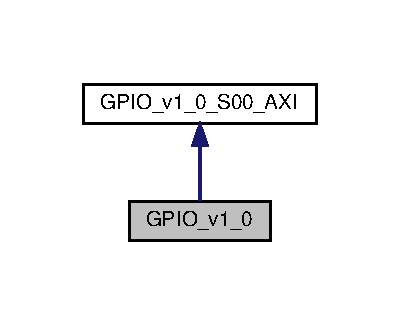
\includegraphics[width=192pt]{classGPIO__v1__0__inherit__graph}
\end{center}
\end{figure}


Collaboration diagram for G\+P\+I\+O\+\_\+v1\+\_\+0\+:\nopagebreak
\begin{figure}[H]
\begin{center}
\leavevmode
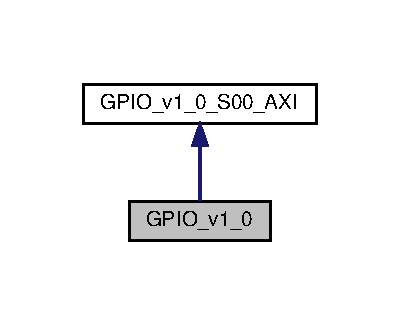
\includegraphics[width=192pt]{classGPIO__v1__0__coll__graph}
\end{center}
\end{figure}
\subsection*{Entities}
\begin{DoxyCompactItemize}
\item 
\hyperlink{classGPIO__v1__0_1_1arch__imp}{arch\+\_\+imp} architecture
\end{DoxyCompactItemize}
\subsection*{Libraries}
 \begin{DoxyCompactItemize}
\item 
\mbox{\Hypertarget{classGPIO__v1__0_a0a6af6eef40212dbaf130d57ce711256}\label{classGPIO__v1__0_a0a6af6eef40212dbaf130d57ce711256}} 
\hyperlink{classGPIO__v1__0_a0a6af6eef40212dbaf130d57ce711256}{ieee} 
\begin{DoxyCompactList}\small\item\em Viene utilizzata la libreria I\+E\+EE. \end{DoxyCompactList}\end{DoxyCompactItemize}
\subsection*{Use Clauses}
 \begin{DoxyCompactItemize}
\item 
\mbox{\Hypertarget{classGPIO__v1__0_acd03516902501cd1c7296a98e22c6fcb}\label{classGPIO__v1__0_acd03516902501cd1c7296a98e22c6fcb}} 
\hyperlink{classGPIO__v1__0_acd03516902501cd1c7296a98e22c6fcb}{std\+\_\+logic\+\_\+1164}   
\begin{DoxyCompactList}\small\item\em Sono utilizzati i segnali della standard logic. \end{DoxyCompactList}\item 
\mbox{\Hypertarget{classGPIO__v1__0_a2edc34402b573437d5f25fa90ba4013e}\label{classGPIO__v1__0_a2edc34402b573437d5f25fa90ba4013e}} 
\hyperlink{classGPIO__v1__0_a2edc34402b573437d5f25fa90ba4013e}{numeric\+\_\+std}   
\begin{DoxyCompactList}\small\item\em Vengono utilizzate le funzioni numeriche. \end{DoxyCompactList}\end{DoxyCompactItemize}
\subsection*{Generics}
 \begin{DoxyCompactItemize}
\item 
\mbox{\Hypertarget{classGPIO__v1__0_a16bbf9205afa677edb8a74dcd39ebb9f}\label{classGPIO__v1__0_a16bbf9205afa677edb8a74dcd39ebb9f}} 
\hyperlink{classGPIO__v1__0_a16bbf9205afa677edb8a74dcd39ebb9f}{width} {\bfseries {\bfseries \textcolor{vhdlchar}{integer}\textcolor{vhdlchar}{ }\textcolor{vhdlchar}{ }\textcolor{vhdlchar}{\+:}\textcolor{vhdlchar}{=}\textcolor{vhdlchar}{ }\textcolor{vhdlchar}{ } \textcolor{vhdldigit}{4} \textcolor{vhdlchar}{ }}}
\begin{DoxyCompactList}\small\item\em determina il numero di \hyperlink{structGPIO}{G\+P\+IO} da controllare \end{DoxyCompactList}\item 
\mbox{\Hypertarget{classGPIO__v1__0_afce7943994a4ddfa81f224225976a4c7}\label{classGPIO__v1__0_afce7943994a4ddfa81f224225976a4c7}} 
\hyperlink{classGPIO__v1__0_afce7943994a4ddfa81f224225976a4c7}{C\+\_\+\+S00\+\_\+\+A\+X\+I\+\_\+\+D\+A\+T\+A\+\_\+\+W\+I\+D\+TH} {\bfseries {\bfseries \textcolor{vhdlchar}{integer}\textcolor{vhdlchar}{ }\textcolor{vhdlchar}{ }\textcolor{vhdlchar}{\+:}\textcolor{vhdlchar}{=}\textcolor{vhdlchar}{ }\textcolor{vhdlchar}{ } \textcolor{vhdldigit}{32} \textcolor{vhdlchar}{ }}}
\item 
\mbox{\Hypertarget{classGPIO__v1__0_ab7787f274c76bb896ac98fdcfb570c65}\label{classGPIO__v1__0_ab7787f274c76bb896ac98fdcfb570c65}} 
\hyperlink{classGPIO__v1__0_ab7787f274c76bb896ac98fdcfb570c65}{C\+\_\+\+S00\+\_\+\+A\+X\+I\+\_\+\+A\+D\+D\+R\+\_\+\+W\+I\+D\+TH} {\bfseries {\bfseries \textcolor{vhdlchar}{integer}\textcolor{vhdlchar}{ }\textcolor{vhdlchar}{ }\textcolor{vhdlchar}{\+:}\textcolor{vhdlchar}{=}\textcolor{vhdlchar}{ }\textcolor{vhdlchar}{ } \textcolor{vhdldigit}{5} \textcolor{vhdlchar}{ }}}
\end{DoxyCompactItemize}
\subsection*{Ports}
 \begin{DoxyCompactItemize}
\item 
\mbox{\Hypertarget{classGPIO__v1__0_ac0744a550c27f11ab186fd7a1156a54e}\label{classGPIO__v1__0_ac0744a550c27f11ab186fd7a1156a54e}} 
\hyperlink{classGPIO__v1__0_ac0744a550c27f11ab186fd7a1156a54e}{pads}  {\bfseries {\bfseries \textcolor{vhdlchar}{inout}\textcolor{vhdlchar}{ }}} {\bfseries \textcolor{vhdlchar}{std\+\_\+logic\+\_\+vector}\textcolor{vhdlchar}{ }\textcolor{vhdlchar}{(}\textcolor{vhdlchar}{ }\textcolor{vhdlchar}{ }\textcolor{vhdlchar}{ }\textcolor{vhdlchar}{ }{\bfseries \hyperlink{classGPIO__v1__0_a16bbf9205afa677edb8a74dcd39ebb9f}{width}} \textcolor{vhdlchar}{-\/}\textcolor{vhdlchar}{ } \textcolor{vhdldigit}{1} \textcolor{vhdlchar}{ }\textcolor{vhdlchar}{downto}\textcolor{vhdlchar}{ }\textcolor{vhdlchar}{ } \textcolor{vhdldigit}{0} \textcolor{vhdlchar}{ }\textcolor{vhdlchar}{)}\textcolor{vhdlchar}{ }} 
\begin{DoxyCompactList}\small\item\em se \hyperlink{structGPIO}{G\+P\+IO} in modalità lettura mostra il valore letto, altrimenti forza un valore in uscita \end{DoxyCompactList}\item 
\mbox{\Hypertarget{classGPIO__v1__0_a5b78f3e3edfaf6e8ec79031b9e631e9d}\label{classGPIO__v1__0_a5b78f3e3edfaf6e8ec79031b9e631e9d}} 
\hyperlink{classGPIO__v1__0_a5b78f3e3edfaf6e8ec79031b9e631e9d}{interrupt}  {\bfseries {\bfseries \textcolor{vhdlchar}{out}\textcolor{vhdlchar}{ }}} {\bfseries \textcolor{vhdlchar}{std\+\_\+logic}\textcolor{vhdlchar}{ }} 
\begin{DoxyCompactList}\small\item\em segnale di interrupt \end{DoxyCompactList}\item 
\mbox{\Hypertarget{classGPIO__v1__0_a037f9e3df8559bfd59db37bcba9cb7a8}\label{classGPIO__v1__0_a037f9e3df8559bfd59db37bcba9cb7a8}} 
\hyperlink{classGPIO__v1__0_a037f9e3df8559bfd59db37bcba9cb7a8}{s00\+\_\+axi\+\_\+aclk}  {\bfseries {\bfseries \textcolor{vhdlchar}{in}\textcolor{vhdlchar}{ }}} {\bfseries \textcolor{vhdlchar}{std\+\_\+logic}\textcolor{vhdlchar}{ }} 
\item 
\mbox{\Hypertarget{classGPIO__v1__0_a8249c106fbd80196dcad2666c9f0b3fc}\label{classGPIO__v1__0_a8249c106fbd80196dcad2666c9f0b3fc}} 
\hyperlink{classGPIO__v1__0_a8249c106fbd80196dcad2666c9f0b3fc}{s00\+\_\+axi\+\_\+aresetn}  {\bfseries {\bfseries \textcolor{vhdlchar}{in}\textcolor{vhdlchar}{ }}} {\bfseries \textcolor{vhdlchar}{std\+\_\+logic}\textcolor{vhdlchar}{ }} 
\item 
\mbox{\Hypertarget{classGPIO__v1__0_a9fe80d3cc7f862afb670536e4e05dbeb}\label{classGPIO__v1__0_a9fe80d3cc7f862afb670536e4e05dbeb}} 
\hyperlink{classGPIO__v1__0_a9fe80d3cc7f862afb670536e4e05dbeb}{s00\+\_\+axi\+\_\+awaddr}  {\bfseries {\bfseries \textcolor{vhdlchar}{in}\textcolor{vhdlchar}{ }}} {\bfseries \textcolor{vhdlchar}{std\+\_\+logic\+\_\+vector}\textcolor{vhdlchar}{ }\textcolor{vhdlchar}{(}\textcolor{vhdlchar}{ }\textcolor{vhdlchar}{ }\textcolor{vhdlchar}{ }\textcolor{vhdlchar}{ }\textcolor{vhdlchar}{C\+\_\+\+S00\+\_\+\+A\+X\+I\+\_\+\+A\+D\+D\+R\+\_\+\+W\+I\+D\+TH}\textcolor{vhdlchar}{-\/}\textcolor{vhdlchar}{ } \textcolor{vhdldigit}{1} \textcolor{vhdlchar}{ }\textcolor{vhdlchar}{downto}\textcolor{vhdlchar}{ }\textcolor{vhdlchar}{ } \textcolor{vhdldigit}{0} \textcolor{vhdlchar}{ }\textcolor{vhdlchar}{)}\textcolor{vhdlchar}{ }} 
\item 
\mbox{\Hypertarget{classGPIO__v1__0_a719659c1addef5432978cc949d9e10ed}\label{classGPIO__v1__0_a719659c1addef5432978cc949d9e10ed}} 
\hyperlink{classGPIO__v1__0_a719659c1addef5432978cc949d9e10ed}{s00\+\_\+axi\+\_\+awprot}  {\bfseries {\bfseries \textcolor{vhdlchar}{in}\textcolor{vhdlchar}{ }}} {\bfseries \textcolor{vhdlchar}{std\+\_\+logic\+\_\+vector}\textcolor{vhdlchar}{ }\textcolor{vhdlchar}{(}\textcolor{vhdlchar}{ }\textcolor{vhdlchar}{ } \textcolor{vhdldigit}{2} \textcolor{vhdlchar}{ }\textcolor{vhdlchar}{downto}\textcolor{vhdlchar}{ }\textcolor{vhdlchar}{ } \textcolor{vhdldigit}{0} \textcolor{vhdlchar}{ }\textcolor{vhdlchar}{)}\textcolor{vhdlchar}{ }} 
\item 
\mbox{\Hypertarget{classGPIO__v1__0_a45aa02a72ae1a8389346d47173c60ed0}\label{classGPIO__v1__0_a45aa02a72ae1a8389346d47173c60ed0}} 
\hyperlink{classGPIO__v1__0_a45aa02a72ae1a8389346d47173c60ed0}{s00\+\_\+axi\+\_\+awvalid}  {\bfseries {\bfseries \textcolor{vhdlchar}{in}\textcolor{vhdlchar}{ }}} {\bfseries \textcolor{vhdlchar}{std\+\_\+logic}\textcolor{vhdlchar}{ }} 
\item 
\mbox{\Hypertarget{classGPIO__v1__0_ad0a1f71502d91a45dbc6c365f85c6566}\label{classGPIO__v1__0_ad0a1f71502d91a45dbc6c365f85c6566}} 
\hyperlink{classGPIO__v1__0_ad0a1f71502d91a45dbc6c365f85c6566}{s00\+\_\+axi\+\_\+awready}  {\bfseries {\bfseries \textcolor{vhdlchar}{out}\textcolor{vhdlchar}{ }}} {\bfseries \textcolor{vhdlchar}{std\+\_\+logic}\textcolor{vhdlchar}{ }} 
\item 
\mbox{\Hypertarget{classGPIO__v1__0_ae2b15b55ee463fd9dd030ee29db6bb17}\label{classGPIO__v1__0_ae2b15b55ee463fd9dd030ee29db6bb17}} 
\hyperlink{classGPIO__v1__0_ae2b15b55ee463fd9dd030ee29db6bb17}{s00\+\_\+axi\+\_\+wdata}  {\bfseries {\bfseries \textcolor{vhdlchar}{in}\textcolor{vhdlchar}{ }}} {\bfseries \textcolor{vhdlchar}{std\+\_\+logic\+\_\+vector}\textcolor{vhdlchar}{ }\textcolor{vhdlchar}{(}\textcolor{vhdlchar}{ }\textcolor{vhdlchar}{ }\textcolor{vhdlchar}{ }\textcolor{vhdlchar}{ }\textcolor{vhdlchar}{C\+\_\+\+S00\+\_\+\+A\+X\+I\+\_\+\+D\+A\+T\+A\+\_\+\+W\+I\+D\+TH}\textcolor{vhdlchar}{-\/}\textcolor{vhdlchar}{ } \textcolor{vhdldigit}{1} \textcolor{vhdlchar}{ }\textcolor{vhdlchar}{downto}\textcolor{vhdlchar}{ }\textcolor{vhdlchar}{ } \textcolor{vhdldigit}{0} \textcolor{vhdlchar}{ }\textcolor{vhdlchar}{)}\textcolor{vhdlchar}{ }} 
\item 
\mbox{\Hypertarget{classGPIO__v1__0_a120924bc3fd5fd10ec0f96e19c3f4904}\label{classGPIO__v1__0_a120924bc3fd5fd10ec0f96e19c3f4904}} 
\hyperlink{classGPIO__v1__0_a120924bc3fd5fd10ec0f96e19c3f4904}{s00\+\_\+axi\+\_\+wstrb}  {\bfseries {\bfseries \textcolor{vhdlchar}{in}\textcolor{vhdlchar}{ }}} {\bfseries \textcolor{vhdlchar}{std\+\_\+logic\+\_\+vector}\textcolor{vhdlchar}{ }\textcolor{vhdlchar}{(}\textcolor{vhdlchar}{ }\textcolor{vhdlchar}{(}\textcolor{vhdlchar}{ }\textcolor{vhdlchar}{ }\textcolor{vhdlchar}{ }\textcolor{vhdlchar}{ }\textcolor{vhdlchar}{C\+\_\+\+S00\+\_\+\+A\+X\+I\+\_\+\+D\+A\+T\+A\+\_\+\+W\+I\+D\+TH}\textcolor{vhdlchar}{/}\textcolor{vhdlchar}{ } \textcolor{vhdldigit}{8} \textcolor{vhdlchar}{ }\textcolor{vhdlchar}{)}\textcolor{vhdlchar}{ }\textcolor{vhdlchar}{-\/}\textcolor{vhdlchar}{ } \textcolor{vhdldigit}{1} \textcolor{vhdlchar}{ }\textcolor{vhdlchar}{downto}\textcolor{vhdlchar}{ }\textcolor{vhdlchar}{ } \textcolor{vhdldigit}{0} \textcolor{vhdlchar}{ }\textcolor{vhdlchar}{)}\textcolor{vhdlchar}{ }} 
\item 
\mbox{\Hypertarget{classGPIO__v1__0_a24e90907193647007d2947353740114d}\label{classGPIO__v1__0_a24e90907193647007d2947353740114d}} 
\hyperlink{classGPIO__v1__0_a24e90907193647007d2947353740114d}{s00\+\_\+axi\+\_\+wvalid}  {\bfseries {\bfseries \textcolor{vhdlchar}{in}\textcolor{vhdlchar}{ }}} {\bfseries \textcolor{vhdlchar}{std\+\_\+logic}\textcolor{vhdlchar}{ }} 
\item 
\mbox{\Hypertarget{classGPIO__v1__0_a3fc60abc0cfbfa90003a83bffdd476c4}\label{classGPIO__v1__0_a3fc60abc0cfbfa90003a83bffdd476c4}} 
\hyperlink{classGPIO__v1__0_a3fc60abc0cfbfa90003a83bffdd476c4}{s00\+\_\+axi\+\_\+wready}  {\bfseries {\bfseries \textcolor{vhdlchar}{out}\textcolor{vhdlchar}{ }}} {\bfseries \textcolor{vhdlchar}{std\+\_\+logic}\textcolor{vhdlchar}{ }} 
\item 
\mbox{\Hypertarget{classGPIO__v1__0_af8799be946d3f5354263e7deb15f94f1}\label{classGPIO__v1__0_af8799be946d3f5354263e7deb15f94f1}} 
\hyperlink{classGPIO__v1__0_af8799be946d3f5354263e7deb15f94f1}{s00\+\_\+axi\+\_\+bresp}  {\bfseries {\bfseries \textcolor{vhdlchar}{out}\textcolor{vhdlchar}{ }}} {\bfseries \textcolor{vhdlchar}{std\+\_\+logic\+\_\+vector}\textcolor{vhdlchar}{ }\textcolor{vhdlchar}{(}\textcolor{vhdlchar}{ }\textcolor{vhdlchar}{ } \textcolor{vhdldigit}{1} \textcolor{vhdlchar}{ }\textcolor{vhdlchar}{downto}\textcolor{vhdlchar}{ }\textcolor{vhdlchar}{ } \textcolor{vhdldigit}{0} \textcolor{vhdlchar}{ }\textcolor{vhdlchar}{)}\textcolor{vhdlchar}{ }} 
\item 
\mbox{\Hypertarget{classGPIO__v1__0_a5110b7dd4fb9548a2aab88f50dbe1d5e}\label{classGPIO__v1__0_a5110b7dd4fb9548a2aab88f50dbe1d5e}} 
\hyperlink{classGPIO__v1__0_a5110b7dd4fb9548a2aab88f50dbe1d5e}{s00\+\_\+axi\+\_\+bvalid}  {\bfseries {\bfseries \textcolor{vhdlchar}{out}\textcolor{vhdlchar}{ }}} {\bfseries \textcolor{vhdlchar}{std\+\_\+logic}\textcolor{vhdlchar}{ }} 
\item 
\mbox{\Hypertarget{classGPIO__v1__0_a1ef2019b0613bc23d4829eeeb24eb98d}\label{classGPIO__v1__0_a1ef2019b0613bc23d4829eeeb24eb98d}} 
\hyperlink{classGPIO__v1__0_a1ef2019b0613bc23d4829eeeb24eb98d}{s00\+\_\+axi\+\_\+bready}  {\bfseries {\bfseries \textcolor{vhdlchar}{in}\textcolor{vhdlchar}{ }}} {\bfseries \textcolor{vhdlchar}{std\+\_\+logic}\textcolor{vhdlchar}{ }} 
\item 
\mbox{\Hypertarget{classGPIO__v1__0_af70a86336cd6505064e45b69f4623939}\label{classGPIO__v1__0_af70a86336cd6505064e45b69f4623939}} 
\hyperlink{classGPIO__v1__0_af70a86336cd6505064e45b69f4623939}{s00\+\_\+axi\+\_\+araddr}  {\bfseries {\bfseries \textcolor{vhdlchar}{in}\textcolor{vhdlchar}{ }}} {\bfseries \textcolor{vhdlchar}{std\+\_\+logic\+\_\+vector}\textcolor{vhdlchar}{ }\textcolor{vhdlchar}{(}\textcolor{vhdlchar}{ }\textcolor{vhdlchar}{ }\textcolor{vhdlchar}{ }\textcolor{vhdlchar}{ }\textcolor{vhdlchar}{C\+\_\+\+S00\+\_\+\+A\+X\+I\+\_\+\+A\+D\+D\+R\+\_\+\+W\+I\+D\+TH}\textcolor{vhdlchar}{-\/}\textcolor{vhdlchar}{ } \textcolor{vhdldigit}{1} \textcolor{vhdlchar}{ }\textcolor{vhdlchar}{downto}\textcolor{vhdlchar}{ }\textcolor{vhdlchar}{ } \textcolor{vhdldigit}{0} \textcolor{vhdlchar}{ }\textcolor{vhdlchar}{)}\textcolor{vhdlchar}{ }} 
\item 
\mbox{\Hypertarget{classGPIO__v1__0_adc648df07895bf808b8c721e1dc6811b}\label{classGPIO__v1__0_adc648df07895bf808b8c721e1dc6811b}} 
\hyperlink{classGPIO__v1__0_adc648df07895bf808b8c721e1dc6811b}{s00\+\_\+axi\+\_\+arprot}  {\bfseries {\bfseries \textcolor{vhdlchar}{in}\textcolor{vhdlchar}{ }}} {\bfseries \textcolor{vhdlchar}{std\+\_\+logic\+\_\+vector}\textcolor{vhdlchar}{ }\textcolor{vhdlchar}{(}\textcolor{vhdlchar}{ }\textcolor{vhdlchar}{ } \textcolor{vhdldigit}{2} \textcolor{vhdlchar}{ }\textcolor{vhdlchar}{downto}\textcolor{vhdlchar}{ }\textcolor{vhdlchar}{ } \textcolor{vhdldigit}{0} \textcolor{vhdlchar}{ }\textcolor{vhdlchar}{)}\textcolor{vhdlchar}{ }} 
\item 
\mbox{\Hypertarget{classGPIO__v1__0_a94b78b2ae3cd13860f15afbdfb199e44}\label{classGPIO__v1__0_a94b78b2ae3cd13860f15afbdfb199e44}} 
\hyperlink{classGPIO__v1__0_a94b78b2ae3cd13860f15afbdfb199e44}{s00\+\_\+axi\+\_\+arvalid}  {\bfseries {\bfseries \textcolor{vhdlchar}{in}\textcolor{vhdlchar}{ }}} {\bfseries \textcolor{vhdlchar}{std\+\_\+logic}\textcolor{vhdlchar}{ }} 
\item 
\mbox{\Hypertarget{classGPIO__v1__0_ad35bd95f3352ff8dbdaea55205a98e53}\label{classGPIO__v1__0_ad35bd95f3352ff8dbdaea55205a98e53}} 
\hyperlink{classGPIO__v1__0_ad35bd95f3352ff8dbdaea55205a98e53}{s00\+\_\+axi\+\_\+arready}  {\bfseries {\bfseries \textcolor{vhdlchar}{out}\textcolor{vhdlchar}{ }}} {\bfseries \textcolor{vhdlchar}{std\+\_\+logic}\textcolor{vhdlchar}{ }} 
\item 
\mbox{\Hypertarget{classGPIO__v1__0_ad2655fadb987e0487c428aca187b55d0}\label{classGPIO__v1__0_ad2655fadb987e0487c428aca187b55d0}} 
\hyperlink{classGPIO__v1__0_ad2655fadb987e0487c428aca187b55d0}{s00\+\_\+axi\+\_\+rdata}  {\bfseries {\bfseries \textcolor{vhdlchar}{out}\textcolor{vhdlchar}{ }}} {\bfseries \textcolor{vhdlchar}{std\+\_\+logic\+\_\+vector}\textcolor{vhdlchar}{ }\textcolor{vhdlchar}{(}\textcolor{vhdlchar}{ }\textcolor{vhdlchar}{ }\textcolor{vhdlchar}{ }\textcolor{vhdlchar}{ }\textcolor{vhdlchar}{C\+\_\+\+S00\+\_\+\+A\+X\+I\+\_\+\+D\+A\+T\+A\+\_\+\+W\+I\+D\+TH}\textcolor{vhdlchar}{-\/}\textcolor{vhdlchar}{ } \textcolor{vhdldigit}{1} \textcolor{vhdlchar}{ }\textcolor{vhdlchar}{downto}\textcolor{vhdlchar}{ }\textcolor{vhdlchar}{ } \textcolor{vhdldigit}{0} \textcolor{vhdlchar}{ }\textcolor{vhdlchar}{)}\textcolor{vhdlchar}{ }} 
\item 
\mbox{\Hypertarget{classGPIO__v1__0_a1acee955f50f71e5595a03c6ca301cf0}\label{classGPIO__v1__0_a1acee955f50f71e5595a03c6ca301cf0}} 
\hyperlink{classGPIO__v1__0_a1acee955f50f71e5595a03c6ca301cf0}{s00\+\_\+axi\+\_\+rresp}  {\bfseries {\bfseries \textcolor{vhdlchar}{out}\textcolor{vhdlchar}{ }}} {\bfseries \textcolor{vhdlchar}{std\+\_\+logic\+\_\+vector}\textcolor{vhdlchar}{ }\textcolor{vhdlchar}{(}\textcolor{vhdlchar}{ }\textcolor{vhdlchar}{ } \textcolor{vhdldigit}{1} \textcolor{vhdlchar}{ }\textcolor{vhdlchar}{downto}\textcolor{vhdlchar}{ }\textcolor{vhdlchar}{ } \textcolor{vhdldigit}{0} \textcolor{vhdlchar}{ }\textcolor{vhdlchar}{)}\textcolor{vhdlchar}{ }} 
\item 
\mbox{\Hypertarget{classGPIO__v1__0_af180911f7eb262e530e26865bc97aa0b}\label{classGPIO__v1__0_af180911f7eb262e530e26865bc97aa0b}} 
\hyperlink{classGPIO__v1__0_af180911f7eb262e530e26865bc97aa0b}{s00\+\_\+axi\+\_\+rvalid}  {\bfseries {\bfseries \textcolor{vhdlchar}{out}\textcolor{vhdlchar}{ }}} {\bfseries \textcolor{vhdlchar}{std\+\_\+logic}\textcolor{vhdlchar}{ }} 
\item 
\mbox{\Hypertarget{classGPIO__v1__0_a8b82eb165d7024f6c7b25646f6ebdd4d}\label{classGPIO__v1__0_a8b82eb165d7024f6c7b25646f6ebdd4d}} 
\hyperlink{classGPIO__v1__0_a8b82eb165d7024f6c7b25646f6ebdd4d}{s00\+\_\+axi\+\_\+rready}  {\bfseries {\bfseries \textcolor{vhdlchar}{in}\textcolor{vhdlchar}{ }}} {\bfseries \textcolor{vhdlchar}{std\+\_\+logic}\textcolor{vhdlchar}{ }} 
\end{DoxyCompactItemize}


The documentation for this class was generated from the following file\+:\begin{DoxyCompactItemize}
\item 
/media/saverio/\+O\+S/\+Users/\+Saverio/\+Desktop/\+S\+E/git/codici\+\_\+da\+\_\+mandare/\+F\+P\+G\+A/\+G\+P\+I\+O/\+Hardware/\+G\+P\+I\+O\+\_\+1.\+0/hdl/\hyperlink{GPIO__v1__0_8vhd}{G\+P\+I\+O\+\_\+v1\+\_\+0.\+vhd}\end{DoxyCompactItemize}

\hypertarget{classGPIO__v1__0__S00__AXI}{}\section{G\+P\+I\+O\+\_\+v1\+\_\+0\+\_\+\+S00\+\_\+\+A\+XI Entity Reference}
\label{classGPIO__v1__0__S00__AXI}\index{G\+P\+I\+O\+\_\+v1\+\_\+0\+\_\+\+S00\+\_\+\+A\+XI@{G\+P\+I\+O\+\_\+v1\+\_\+0\+\_\+\+S00\+\_\+\+A\+XI}}


Inheritance diagram for G\+P\+I\+O\+\_\+v1\+\_\+0\+\_\+\+S00\+\_\+\+A\+XI\+:\nopagebreak
\begin{figure}[H]
\begin{center}
\leavevmode
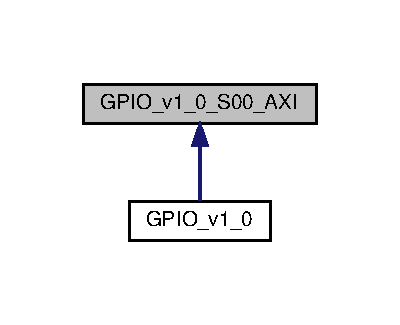
\includegraphics[width=192pt]{classGPIO__v1__0__S00__AXI__inherit__graph}
\end{center}
\end{figure}
\subsection*{Entities}
\begin{DoxyCompactItemize}
\item 
\hyperlink{classGPIO__v1__0__S00__AXI_1_1arch__imp}{arch\+\_\+imp} architecture
\end{DoxyCompactItemize}
\subsection*{Libraries}
 \begin{DoxyCompactItemize}
\item 
\mbox{\Hypertarget{classGPIO__v1__0__S00__AXI_a0a6af6eef40212dbaf130d57ce711256}\label{classGPIO__v1__0__S00__AXI_a0a6af6eef40212dbaf130d57ce711256}} 
\hyperlink{classGPIO__v1__0__S00__AXI_a0a6af6eef40212dbaf130d57ce711256}{ieee} 
\begin{DoxyCompactList}\small\item\em Viene utilizzato la libreria I\+E\+EE. \end{DoxyCompactList}\end{DoxyCompactItemize}
\subsection*{Use Clauses}
 \begin{DoxyCompactItemize}
\item 
\mbox{\Hypertarget{classGPIO__v1__0__S00__AXI_acd03516902501cd1c7296a98e22c6fcb}\label{classGPIO__v1__0__S00__AXI_acd03516902501cd1c7296a98e22c6fcb}} 
\hyperlink{classGPIO__v1__0__S00__AXI_acd03516902501cd1c7296a98e22c6fcb}{std\+\_\+logic\+\_\+1164}   
\begin{DoxyCompactList}\small\item\em Sono utilizzati i segnali della standard logic. \end{DoxyCompactList}\item 
\mbox{\Hypertarget{classGPIO__v1__0__S00__AXI_a2edc34402b573437d5f25fa90ba4013e}\label{classGPIO__v1__0__S00__AXI_a2edc34402b573437d5f25fa90ba4013e}} 
\hyperlink{classGPIO__v1__0__S00__AXI_a2edc34402b573437d5f25fa90ba4013e}{numeric\+\_\+std}   
\begin{DoxyCompactList}\small\item\em Vengono utilizzate le funzioni numeriche. \end{DoxyCompactList}\item 
\mbox{\Hypertarget{classGPIO__v1__0__S00__AXI_acb2d98d781f19c8f5f4109576ec45502}\label{classGPIO__v1__0__S00__AXI_acb2d98d781f19c8f5f4109576ec45502}} 
\hyperlink{classGPIO__v1__0__S00__AXI_acb2d98d781f19c8f5f4109576ec45502}{std\+\_\+logic\+\_\+misc}   
\begin{DoxyCompactList}\small\item\em Viene utilizzata la libreria misc di utility. \end{DoxyCompactList}\end{DoxyCompactItemize}
\subsection*{Generics}
 \begin{DoxyCompactItemize}
\item 
\mbox{\Hypertarget{classGPIO__v1__0__S00__AXI_a16bbf9205afa677edb8a74dcd39ebb9f}\label{classGPIO__v1__0__S00__AXI_a16bbf9205afa677edb8a74dcd39ebb9f}} 
\hyperlink{classGPIO__v1__0__S00__AXI_a16bbf9205afa677edb8a74dcd39ebb9f}{width} {\bfseries {\bfseries \textcolor{vhdlchar}{integer}\textcolor{vhdlchar}{ }\textcolor{vhdlchar}{ }\textcolor{vhdlchar}{\+:}\textcolor{vhdlchar}{=}\textcolor{vhdlchar}{ }\textcolor{vhdlchar}{ } \textcolor{vhdldigit}{4} \textcolor{vhdlchar}{ }}}
\begin{DoxyCompactList}\small\item\em determina il numero di \hyperlink{structGPIO}{G\+P\+IO} da controllare \end{DoxyCompactList}\item 
\mbox{\Hypertarget{classGPIO__v1__0__S00__AXI_a0fad312acd1f302ce7de30c5658df0bd}\label{classGPIO__v1__0__S00__AXI_a0fad312acd1f302ce7de30c5658df0bd}} 
\hyperlink{classGPIO__v1__0__S00__AXI_a0fad312acd1f302ce7de30c5658df0bd}{C\+\_\+\+S\+\_\+\+A\+X\+I\+\_\+\+D\+A\+T\+A\+\_\+\+W\+I\+D\+TH} {\bfseries {\bfseries \textcolor{vhdlchar}{integer}\textcolor{vhdlchar}{ }\textcolor{vhdlchar}{ }\textcolor{vhdlchar}{\+:}\textcolor{vhdlchar}{=}\textcolor{vhdlchar}{ }\textcolor{vhdlchar}{ } \textcolor{vhdldigit}{32} \textcolor{vhdlchar}{ }}}
\item 
\mbox{\Hypertarget{classGPIO__v1__0__S00__AXI_a9abff2eaa069440f3b7d9e9937d5ee8e}\label{classGPIO__v1__0__S00__AXI_a9abff2eaa069440f3b7d9e9937d5ee8e}} 
\hyperlink{classGPIO__v1__0__S00__AXI_a9abff2eaa069440f3b7d9e9937d5ee8e}{C\+\_\+\+S\+\_\+\+A\+X\+I\+\_\+\+A\+D\+D\+R\+\_\+\+W\+I\+D\+TH} {\bfseries {\bfseries \textcolor{vhdlchar}{integer}\textcolor{vhdlchar}{ }\textcolor{vhdlchar}{ }\textcolor{vhdlchar}{\+:}\textcolor{vhdlchar}{=}\textcolor{vhdlchar}{ }\textcolor{vhdlchar}{ } \textcolor{vhdldigit}{5} \textcolor{vhdlchar}{ }}}
\end{DoxyCompactItemize}
\subsection*{Ports}
 \begin{DoxyCompactItemize}
\item 
\mbox{\Hypertarget{classGPIO__v1__0__S00__AXI_ac0744a550c27f11ab186fd7a1156a54e}\label{classGPIO__v1__0__S00__AXI_ac0744a550c27f11ab186fd7a1156a54e}} 
\hyperlink{classGPIO__v1__0__S00__AXI_ac0744a550c27f11ab186fd7a1156a54e}{pads}  {\bfseries {\bfseries \textcolor{vhdlchar}{inout}\textcolor{vhdlchar}{ }}} {\bfseries \textcolor{vhdlchar}{std\+\_\+logic\+\_\+vector}\textcolor{vhdlchar}{ }\textcolor{vhdlchar}{(}\textcolor{vhdlchar}{ }\textcolor{vhdlchar}{ }\textcolor{vhdlchar}{ }\textcolor{vhdlchar}{ }{\bfseries \hyperlink{classGPIO__v1__0__S00__AXI_a16bbf9205afa677edb8a74dcd39ebb9f}{width}} \textcolor{vhdlchar}{-\/}\textcolor{vhdlchar}{ } \textcolor{vhdldigit}{1} \textcolor{vhdlchar}{ }\textcolor{vhdlchar}{downto}\textcolor{vhdlchar}{ }\textcolor{vhdlchar}{ } \textcolor{vhdldigit}{0} \textcolor{vhdlchar}{ }\textcolor{vhdlchar}{)}\textcolor{vhdlchar}{ }} 
\begin{DoxyCompactList}\small\item\em se \hyperlink{structGPIO}{G\+P\+IO} in modalità lettura mostra il valore letto, altrimenti forza un valore in uscita \end{DoxyCompactList}\item 
\mbox{\Hypertarget{classGPIO__v1__0__S00__AXI_a5b78f3e3edfaf6e8ec79031b9e631e9d}\label{classGPIO__v1__0__S00__AXI_a5b78f3e3edfaf6e8ec79031b9e631e9d}} 
\hyperlink{classGPIO__v1__0__S00__AXI_a5b78f3e3edfaf6e8ec79031b9e631e9d}{interrupt}  {\bfseries {\bfseries \textcolor{vhdlchar}{out}\textcolor{vhdlchar}{ }}} {\bfseries \textcolor{vhdlchar}{std\+\_\+logic}\textcolor{vhdlchar}{ }} 
\begin{DoxyCompactList}\small\item\em segnale di interrupt \end{DoxyCompactList}\item 
\mbox{\Hypertarget{classGPIO__v1__0__S00__AXI_a3f54d782a88290bdaa6baffd7cd84ab4}\label{classGPIO__v1__0__S00__AXI_a3f54d782a88290bdaa6baffd7cd84ab4}} 
\hyperlink{classGPIO__v1__0__S00__AXI_a3f54d782a88290bdaa6baffd7cd84ab4}{S\+\_\+\+A\+X\+I\+\_\+\+A\+C\+LK}  {\bfseries {\bfseries \textcolor{vhdlchar}{in}\textcolor{vhdlchar}{ }}} {\bfseries \textcolor{vhdlchar}{std\+\_\+logic}\textcolor{vhdlchar}{ }} 
\item 
\mbox{\Hypertarget{classGPIO__v1__0__S00__AXI_a089b396e17dee353ccc7d5389dda5532}\label{classGPIO__v1__0__S00__AXI_a089b396e17dee353ccc7d5389dda5532}} 
\hyperlink{classGPIO__v1__0__S00__AXI_a089b396e17dee353ccc7d5389dda5532}{S\+\_\+\+A\+X\+I\+\_\+\+A\+R\+E\+S\+E\+TN}  {\bfseries {\bfseries \textcolor{vhdlchar}{in}\textcolor{vhdlchar}{ }}} {\bfseries \textcolor{vhdlchar}{std\+\_\+logic}\textcolor{vhdlchar}{ }} 
\item 
\mbox{\Hypertarget{classGPIO__v1__0__S00__AXI_a61cc7b190ba9d540e56941330e4a0883}\label{classGPIO__v1__0__S00__AXI_a61cc7b190ba9d540e56941330e4a0883}} 
\hyperlink{classGPIO__v1__0__S00__AXI_a61cc7b190ba9d540e56941330e4a0883}{S\+\_\+\+A\+X\+I\+\_\+\+A\+W\+A\+D\+DR}  {\bfseries {\bfseries \textcolor{vhdlchar}{in}\textcolor{vhdlchar}{ }}} {\bfseries \textcolor{vhdlchar}{std\+\_\+logic\+\_\+vector}\textcolor{vhdlchar}{ }\textcolor{vhdlchar}{(}\textcolor{vhdlchar}{ }\textcolor{vhdlchar}{ }\textcolor{vhdlchar}{ }\textcolor{vhdlchar}{ }\textcolor{vhdlchar}{C\+\_\+\+S\+\_\+\+A\+X\+I\+\_\+\+A\+D\+D\+R\+\_\+\+W\+I\+D\+TH}\textcolor{vhdlchar}{-\/}\textcolor{vhdlchar}{ } \textcolor{vhdldigit}{1} \textcolor{vhdlchar}{ }\textcolor{vhdlchar}{downto}\textcolor{vhdlchar}{ }\textcolor{vhdlchar}{ } \textcolor{vhdldigit}{0} \textcolor{vhdlchar}{ }\textcolor{vhdlchar}{)}\textcolor{vhdlchar}{ }} 
\item 
\mbox{\Hypertarget{classGPIO__v1__0__S00__AXI_a459abcd98567ad24261377eed899593a}\label{classGPIO__v1__0__S00__AXI_a459abcd98567ad24261377eed899593a}} 
\hyperlink{classGPIO__v1__0__S00__AXI_a459abcd98567ad24261377eed899593a}{S\+\_\+\+A\+X\+I\+\_\+\+A\+W\+P\+R\+OT}  {\bfseries {\bfseries \textcolor{vhdlchar}{in}\textcolor{vhdlchar}{ }}} {\bfseries \textcolor{vhdlchar}{std\+\_\+logic\+\_\+vector}\textcolor{vhdlchar}{ }\textcolor{vhdlchar}{(}\textcolor{vhdlchar}{ }\textcolor{vhdlchar}{ } \textcolor{vhdldigit}{2} \textcolor{vhdlchar}{ }\textcolor{vhdlchar}{downto}\textcolor{vhdlchar}{ }\textcolor{vhdlchar}{ } \textcolor{vhdldigit}{0} \textcolor{vhdlchar}{ }\textcolor{vhdlchar}{)}\textcolor{vhdlchar}{ }} 
\item 
\mbox{\Hypertarget{classGPIO__v1__0__S00__AXI_af1f1cbf67bf647ba58353c261719a3a0}\label{classGPIO__v1__0__S00__AXI_af1f1cbf67bf647ba58353c261719a3a0}} 
\hyperlink{classGPIO__v1__0__S00__AXI_af1f1cbf67bf647ba58353c261719a3a0}{S\+\_\+\+A\+X\+I\+\_\+\+A\+W\+V\+A\+L\+ID}  {\bfseries {\bfseries \textcolor{vhdlchar}{in}\textcolor{vhdlchar}{ }}} {\bfseries \textcolor{vhdlchar}{std\+\_\+logic}\textcolor{vhdlchar}{ }} 
\item 
\mbox{\Hypertarget{classGPIO__v1__0__S00__AXI_ac04aab5cc834e762e893e061016921c6}\label{classGPIO__v1__0__S00__AXI_ac04aab5cc834e762e893e061016921c6}} 
\hyperlink{classGPIO__v1__0__S00__AXI_ac04aab5cc834e762e893e061016921c6}{S\+\_\+\+A\+X\+I\+\_\+\+A\+W\+R\+E\+A\+DY}  {\bfseries {\bfseries \textcolor{vhdlchar}{out}\textcolor{vhdlchar}{ }}} {\bfseries \textcolor{vhdlchar}{std\+\_\+logic}\textcolor{vhdlchar}{ }} 
\item 
\mbox{\Hypertarget{classGPIO__v1__0__S00__AXI_a292e5db13719faf3a8b3aab091773467}\label{classGPIO__v1__0__S00__AXI_a292e5db13719faf3a8b3aab091773467}} 
\hyperlink{classGPIO__v1__0__S00__AXI_a292e5db13719faf3a8b3aab091773467}{S\+\_\+\+A\+X\+I\+\_\+\+W\+D\+A\+TA}  {\bfseries {\bfseries \textcolor{vhdlchar}{in}\textcolor{vhdlchar}{ }}} {\bfseries \textcolor{vhdlchar}{std\+\_\+logic\+\_\+vector}\textcolor{vhdlchar}{ }\textcolor{vhdlchar}{(}\textcolor{vhdlchar}{ }\textcolor{vhdlchar}{ }\textcolor{vhdlchar}{ }\textcolor{vhdlchar}{ }\textcolor{vhdlchar}{C\+\_\+\+S\+\_\+\+A\+X\+I\+\_\+\+D\+A\+T\+A\+\_\+\+W\+I\+D\+TH}\textcolor{vhdlchar}{-\/}\textcolor{vhdlchar}{ } \textcolor{vhdldigit}{1} \textcolor{vhdlchar}{ }\textcolor{vhdlchar}{downto}\textcolor{vhdlchar}{ }\textcolor{vhdlchar}{ } \textcolor{vhdldigit}{0} \textcolor{vhdlchar}{ }\textcolor{vhdlchar}{)}\textcolor{vhdlchar}{ }} 
\item 
\mbox{\Hypertarget{classGPIO__v1__0__S00__AXI_accd8e04b79540b57ab15fee1cb6c04f5}\label{classGPIO__v1__0__S00__AXI_accd8e04b79540b57ab15fee1cb6c04f5}} 
\hyperlink{classGPIO__v1__0__S00__AXI_accd8e04b79540b57ab15fee1cb6c04f5}{S\+\_\+\+A\+X\+I\+\_\+\+W\+S\+T\+RB}  {\bfseries {\bfseries \textcolor{vhdlchar}{in}\textcolor{vhdlchar}{ }}} {\bfseries \textcolor{vhdlchar}{std\+\_\+logic\+\_\+vector}\textcolor{vhdlchar}{ }\textcolor{vhdlchar}{(}\textcolor{vhdlchar}{ }\textcolor{vhdlchar}{(}\textcolor{vhdlchar}{ }\textcolor{vhdlchar}{ }\textcolor{vhdlchar}{ }\textcolor{vhdlchar}{ }\textcolor{vhdlchar}{C\+\_\+\+S\+\_\+\+A\+X\+I\+\_\+\+D\+A\+T\+A\+\_\+\+W\+I\+D\+TH}\textcolor{vhdlchar}{/}\textcolor{vhdlchar}{ } \textcolor{vhdldigit}{8} \textcolor{vhdlchar}{ }\textcolor{vhdlchar}{)}\textcolor{vhdlchar}{ }\textcolor{vhdlchar}{-\/}\textcolor{vhdlchar}{ } \textcolor{vhdldigit}{1} \textcolor{vhdlchar}{ }\textcolor{vhdlchar}{downto}\textcolor{vhdlchar}{ }\textcolor{vhdlchar}{ } \textcolor{vhdldigit}{0} \textcolor{vhdlchar}{ }\textcolor{vhdlchar}{)}\textcolor{vhdlchar}{ }} 
\item 
\mbox{\Hypertarget{classGPIO__v1__0__S00__AXI_a60bd882e2de781af9a7c6c3d494225d5}\label{classGPIO__v1__0__S00__AXI_a60bd882e2de781af9a7c6c3d494225d5}} 
\hyperlink{classGPIO__v1__0__S00__AXI_a60bd882e2de781af9a7c6c3d494225d5}{S\+\_\+\+A\+X\+I\+\_\+\+W\+V\+A\+L\+ID}  {\bfseries {\bfseries \textcolor{vhdlchar}{in}\textcolor{vhdlchar}{ }}} {\bfseries \textcolor{vhdlchar}{std\+\_\+logic}\textcolor{vhdlchar}{ }} 
\item 
\mbox{\Hypertarget{classGPIO__v1__0__S00__AXI_ab84e4db7037141a360c2b59f45124f01}\label{classGPIO__v1__0__S00__AXI_ab84e4db7037141a360c2b59f45124f01}} 
\hyperlink{classGPIO__v1__0__S00__AXI_ab84e4db7037141a360c2b59f45124f01}{S\+\_\+\+A\+X\+I\+\_\+\+W\+R\+E\+A\+DY}  {\bfseries {\bfseries \textcolor{vhdlchar}{out}\textcolor{vhdlchar}{ }}} {\bfseries \textcolor{vhdlchar}{std\+\_\+logic}\textcolor{vhdlchar}{ }} 
\item 
\mbox{\Hypertarget{classGPIO__v1__0__S00__AXI_abca6c9777b38a5a6bc04886924bafcc8}\label{classGPIO__v1__0__S00__AXI_abca6c9777b38a5a6bc04886924bafcc8}} 
\hyperlink{classGPIO__v1__0__S00__AXI_abca6c9777b38a5a6bc04886924bafcc8}{S\+\_\+\+A\+X\+I\+\_\+\+B\+R\+E\+SP}  {\bfseries {\bfseries \textcolor{vhdlchar}{out}\textcolor{vhdlchar}{ }}} {\bfseries \textcolor{vhdlchar}{std\+\_\+logic\+\_\+vector}\textcolor{vhdlchar}{ }\textcolor{vhdlchar}{(}\textcolor{vhdlchar}{ }\textcolor{vhdlchar}{ } \textcolor{vhdldigit}{1} \textcolor{vhdlchar}{ }\textcolor{vhdlchar}{downto}\textcolor{vhdlchar}{ }\textcolor{vhdlchar}{ } \textcolor{vhdldigit}{0} \textcolor{vhdlchar}{ }\textcolor{vhdlchar}{)}\textcolor{vhdlchar}{ }} 
\item 
\mbox{\Hypertarget{classGPIO__v1__0__S00__AXI_a58f260d3ebaa69be91bb65ff9211823b}\label{classGPIO__v1__0__S00__AXI_a58f260d3ebaa69be91bb65ff9211823b}} 
\hyperlink{classGPIO__v1__0__S00__AXI_a58f260d3ebaa69be91bb65ff9211823b}{S\+\_\+\+A\+X\+I\+\_\+\+B\+V\+A\+L\+ID}  {\bfseries {\bfseries \textcolor{vhdlchar}{out}\textcolor{vhdlchar}{ }}} {\bfseries \textcolor{vhdlchar}{std\+\_\+logic}\textcolor{vhdlchar}{ }} 
\item 
\mbox{\Hypertarget{classGPIO__v1__0__S00__AXI_ac265989978a2be832d278f63fc0f06cb}\label{classGPIO__v1__0__S00__AXI_ac265989978a2be832d278f63fc0f06cb}} 
\hyperlink{classGPIO__v1__0__S00__AXI_ac265989978a2be832d278f63fc0f06cb}{S\+\_\+\+A\+X\+I\+\_\+\+B\+R\+E\+A\+DY}  {\bfseries {\bfseries \textcolor{vhdlchar}{in}\textcolor{vhdlchar}{ }}} {\bfseries \textcolor{vhdlchar}{std\+\_\+logic}\textcolor{vhdlchar}{ }} 
\item 
\mbox{\Hypertarget{classGPIO__v1__0__S00__AXI_a4d1dc8ecac269479747e5ac52c70ac45}\label{classGPIO__v1__0__S00__AXI_a4d1dc8ecac269479747e5ac52c70ac45}} 
\hyperlink{classGPIO__v1__0__S00__AXI_a4d1dc8ecac269479747e5ac52c70ac45}{S\+\_\+\+A\+X\+I\+\_\+\+A\+R\+A\+D\+DR}  {\bfseries {\bfseries \textcolor{vhdlchar}{in}\textcolor{vhdlchar}{ }}} {\bfseries \textcolor{vhdlchar}{std\+\_\+logic\+\_\+vector}\textcolor{vhdlchar}{ }\textcolor{vhdlchar}{(}\textcolor{vhdlchar}{ }\textcolor{vhdlchar}{ }\textcolor{vhdlchar}{ }\textcolor{vhdlchar}{ }\textcolor{vhdlchar}{C\+\_\+\+S\+\_\+\+A\+X\+I\+\_\+\+A\+D\+D\+R\+\_\+\+W\+I\+D\+TH}\textcolor{vhdlchar}{-\/}\textcolor{vhdlchar}{ } \textcolor{vhdldigit}{1} \textcolor{vhdlchar}{ }\textcolor{vhdlchar}{downto}\textcolor{vhdlchar}{ }\textcolor{vhdlchar}{ } \textcolor{vhdldigit}{0} \textcolor{vhdlchar}{ }\textcolor{vhdlchar}{)}\textcolor{vhdlchar}{ }} 
\item 
\mbox{\Hypertarget{classGPIO__v1__0__S00__AXI_a30a07c47d3c1182bbb7c904483bb374f}\label{classGPIO__v1__0__S00__AXI_a30a07c47d3c1182bbb7c904483bb374f}} 
\hyperlink{classGPIO__v1__0__S00__AXI_a30a07c47d3c1182bbb7c904483bb374f}{S\+\_\+\+A\+X\+I\+\_\+\+A\+R\+P\+R\+OT}  {\bfseries {\bfseries \textcolor{vhdlchar}{in}\textcolor{vhdlchar}{ }}} {\bfseries \textcolor{vhdlchar}{std\+\_\+logic\+\_\+vector}\textcolor{vhdlchar}{ }\textcolor{vhdlchar}{(}\textcolor{vhdlchar}{ }\textcolor{vhdlchar}{ } \textcolor{vhdldigit}{2} \textcolor{vhdlchar}{ }\textcolor{vhdlchar}{downto}\textcolor{vhdlchar}{ }\textcolor{vhdlchar}{ } \textcolor{vhdldigit}{0} \textcolor{vhdlchar}{ }\textcolor{vhdlchar}{)}\textcolor{vhdlchar}{ }} 
\item 
\mbox{\Hypertarget{classGPIO__v1__0__S00__AXI_a758f6340dd3340ee46deafbae18a47b2}\label{classGPIO__v1__0__S00__AXI_a758f6340dd3340ee46deafbae18a47b2}} 
\hyperlink{classGPIO__v1__0__S00__AXI_a758f6340dd3340ee46deafbae18a47b2}{S\+\_\+\+A\+X\+I\+\_\+\+A\+R\+V\+A\+L\+ID}  {\bfseries {\bfseries \textcolor{vhdlchar}{in}\textcolor{vhdlchar}{ }}} {\bfseries \textcolor{vhdlchar}{std\+\_\+logic}\textcolor{vhdlchar}{ }} 
\item 
\mbox{\Hypertarget{classGPIO__v1__0__S00__AXI_ade4e78e9c32af26578fc5c74ca3197e8}\label{classGPIO__v1__0__S00__AXI_ade4e78e9c32af26578fc5c74ca3197e8}} 
\hyperlink{classGPIO__v1__0__S00__AXI_ade4e78e9c32af26578fc5c74ca3197e8}{S\+\_\+\+A\+X\+I\+\_\+\+A\+R\+R\+E\+A\+DY}  {\bfseries {\bfseries \textcolor{vhdlchar}{out}\textcolor{vhdlchar}{ }}} {\bfseries \textcolor{vhdlchar}{std\+\_\+logic}\textcolor{vhdlchar}{ }} 
\item 
\mbox{\Hypertarget{classGPIO__v1__0__S00__AXI_a194c6eff7c88405e7934dbc2425ee4ab}\label{classGPIO__v1__0__S00__AXI_a194c6eff7c88405e7934dbc2425ee4ab}} 
\hyperlink{classGPIO__v1__0__S00__AXI_a194c6eff7c88405e7934dbc2425ee4ab}{S\+\_\+\+A\+X\+I\+\_\+\+R\+D\+A\+TA}  {\bfseries {\bfseries \textcolor{vhdlchar}{out}\textcolor{vhdlchar}{ }}} {\bfseries \textcolor{vhdlchar}{std\+\_\+logic\+\_\+vector}\textcolor{vhdlchar}{ }\textcolor{vhdlchar}{(}\textcolor{vhdlchar}{ }\textcolor{vhdlchar}{ }\textcolor{vhdlchar}{ }\textcolor{vhdlchar}{ }\textcolor{vhdlchar}{C\+\_\+\+S\+\_\+\+A\+X\+I\+\_\+\+D\+A\+T\+A\+\_\+\+W\+I\+D\+TH}\textcolor{vhdlchar}{-\/}\textcolor{vhdlchar}{ } \textcolor{vhdldigit}{1} \textcolor{vhdlchar}{ }\textcolor{vhdlchar}{downto}\textcolor{vhdlchar}{ }\textcolor{vhdlchar}{ } \textcolor{vhdldigit}{0} \textcolor{vhdlchar}{ }\textcolor{vhdlchar}{)}\textcolor{vhdlchar}{ }} 
\item 
\mbox{\Hypertarget{classGPIO__v1__0__S00__AXI_a67ba85504b4c51fb0eb00d18fd70ad92}\label{classGPIO__v1__0__S00__AXI_a67ba85504b4c51fb0eb00d18fd70ad92}} 
\hyperlink{classGPIO__v1__0__S00__AXI_a67ba85504b4c51fb0eb00d18fd70ad92}{S\+\_\+\+A\+X\+I\+\_\+\+R\+R\+E\+SP}  {\bfseries {\bfseries \textcolor{vhdlchar}{out}\textcolor{vhdlchar}{ }}} {\bfseries \textcolor{vhdlchar}{std\+\_\+logic\+\_\+vector}\textcolor{vhdlchar}{ }\textcolor{vhdlchar}{(}\textcolor{vhdlchar}{ }\textcolor{vhdlchar}{ } \textcolor{vhdldigit}{1} \textcolor{vhdlchar}{ }\textcolor{vhdlchar}{downto}\textcolor{vhdlchar}{ }\textcolor{vhdlchar}{ } \textcolor{vhdldigit}{0} \textcolor{vhdlchar}{ }\textcolor{vhdlchar}{)}\textcolor{vhdlchar}{ }} 
\item 
\mbox{\Hypertarget{classGPIO__v1__0__S00__AXI_a31f4e92d27c2c2005ee5f368a8249604}\label{classGPIO__v1__0__S00__AXI_a31f4e92d27c2c2005ee5f368a8249604}} 
\hyperlink{classGPIO__v1__0__S00__AXI_a31f4e92d27c2c2005ee5f368a8249604}{S\+\_\+\+A\+X\+I\+\_\+\+R\+V\+A\+L\+ID}  {\bfseries {\bfseries \textcolor{vhdlchar}{out}\textcolor{vhdlchar}{ }}} {\bfseries \textcolor{vhdlchar}{std\+\_\+logic}\textcolor{vhdlchar}{ }} 
\item 
\mbox{\Hypertarget{classGPIO__v1__0__S00__AXI_a5850bf8f42acdf01938057507dc703b7}\label{classGPIO__v1__0__S00__AXI_a5850bf8f42acdf01938057507dc703b7}} 
\hyperlink{classGPIO__v1__0__S00__AXI_a5850bf8f42acdf01938057507dc703b7}{S\+\_\+\+A\+X\+I\+\_\+\+R\+R\+E\+A\+DY}  {\bfseries {\bfseries \textcolor{vhdlchar}{in}\textcolor{vhdlchar}{ }}} {\bfseries \textcolor{vhdlchar}{std\+\_\+logic}\textcolor{vhdlchar}{ }} 
\end{DoxyCompactItemize}


The documentation for this class was generated from the following file\+:\begin{DoxyCompactItemize}
\item 
/media/saverio/\+O\+S/\+Users/\+Saverio/\+Desktop/\+S\+E/git/codici\+\_\+da\+\_\+mandare/\+F\+P\+G\+A/\+G\+P\+I\+O/\+Hardware/\+G\+P\+I\+O\+\_\+1.\+0/hdl/\hyperlink{GPIO__v1__0__S00__AXI_8vhd}{G\+P\+I\+O\+\_\+v1\+\_\+0\+\_\+\+S00\+\_\+\+A\+X\+I.\+vhd}\end{DoxyCompactItemize}

\hypertarget{structmyIntGPIO}{}\section{my\+Int\+G\+P\+IO Struct Reference}
\label{structmyIntGPIO}\index{my\+Int\+G\+P\+IO@{my\+Int\+G\+P\+IO}}
\subsection*{Data Fields}


The documentation for this struct was generated from the following file\+:\begin{DoxyCompactItemize}
\item 
/media/saverio/\+O\+S/\+Users/\+Saverio/\+Desktop/\+S\+E/git/codici\+\_\+da\+\_\+mandare/\+F\+P\+G\+A/\+G\+P\+I\+O/\+Hardware/\+G\+P\+I\+O\+With\+Interrupt/\+G\+P\+I\+O\+With\+Interrupt.\+sdk/\+G\+P\+I\+O/src/\hyperlink{gpio__int_8h}{gpio\+\_\+int.\+h}\end{DoxyCompactItemize}

\chapter{File Documentation}
\hypertarget{gpio__int_8c}{}\section{/media/saverio/\+O\+S/\+Users/\+Saverio/\+Desktop/\+S\+E/git/codici\+\_\+da\+\_\+mandare/\+F\+P\+G\+A/\+G\+P\+I\+O/\+Hardware/\+G\+P\+I\+O\+With\+Interrupt/\+G\+P\+I\+O\+With\+Interrupt.sdk/\+G\+P\+I\+O/src/gpio\+\_\+int.c File Reference}
\label{gpio__int_8c}\index{/media/saverio/\+O\+S/\+Users/\+Saverio/\+Desktop/\+S\+E/git/codici\+\_\+da\+\_\+mandare/\+F\+P\+G\+A/\+G\+P\+I\+O/\+Hardware/\+G\+P\+I\+O\+With\+Interrupt/\+G\+P\+I\+O\+With\+Interrupt.\+sdk/\+G\+P\+I\+O/src/gpio\+\_\+int.\+c@{/media/saverio/\+O\+S/\+Users/\+Saverio/\+Desktop/\+S\+E/git/codici\+\_\+da\+\_\+mandare/\+F\+P\+G\+A/\+G\+P\+I\+O/\+Hardware/\+G\+P\+I\+O\+With\+Interrupt/\+G\+P\+I\+O\+With\+Interrupt.\+sdk/\+G\+P\+I\+O/src/gpio\+\_\+int.\+c}}


Funzioni per l\textquotesingle{}utilizzo della periferiferica \hyperlink{structGPIO}{G\+P\+IO}.  




\subsection{Detailed Description}
Funzioni per l\textquotesingle{}utilizzo della periferiferica \hyperlink{structGPIO}{G\+P\+IO}. 



\subsection{Function Documentation}
\mbox{\Hypertarget{gpio__int_8c_a022379c7f96e8c267ae6dde26dfa6a79}\label{gpio__int_8c_a022379c7f96e8c267ae6dde26dfa6a79}} 
\index{gpio\+\_\+int.\+c@{gpio\+\_\+int.\+c}!X\+G\+P\+I\+O\+\_\+\+A\+CK@{X\+G\+P\+I\+O\+\_\+\+A\+CK}}
\index{X\+G\+P\+I\+O\+\_\+\+A\+CK@{X\+G\+P\+I\+O\+\_\+\+A\+CK}!gpio\+\_\+int.\+c@{gpio\+\_\+int.\+c}}
\subsubsection{\texorpdfstring{X\+G\+P\+I\+O\+\_\+\+A\+C\+K()}{XGPIO\_ACK()}}
{\footnotesize\ttfamily void X\+G\+P\+I\+O\+\_\+\+A\+CK (\begin{DoxyParamCaption}\item[{\hyperlink{structmyIntGPIO}{my\+Int\+G\+P\+IO} $\ast$}]{my\+Int\+G\+P\+I\+O\+Instance,  }\item[{u32}]{mask }\end{DoxyParamCaption})}



Permette di dare A\+CK per processare le singole linee di interruzione del componente \hyperlink{structGPIO}{G\+P\+IO}. L\textquotesingle{}A\+CK rimuove la corrisponde interruzione pendente. 


\begin{DoxyParams}{Parameters}
{\em my\+Int\+G\+P\+I\+O\+Instance} & rappresenta la particola instanza del componente \hyperlink{structGPIO}{G\+P\+IO}.\\
\hline
{\em Maschera} & per dare l\textquotesingle{}A\+CK .\\
\hline
\end{DoxyParams}
\begin{DoxyReturn}{Returns}
La corrispondenza bit-\/linea è posizionale. Il valore 1 al bit-\/iesimo indica ack ad interruzione pendente dell\textquotesingle{}iesima linea. 
\end{DoxyReturn}
\mbox{\Hypertarget{gpio__int_8c_abd0d3e890384bbf4d123f09f3e8dfed1}\label{gpio__int_8c_abd0d3e890384bbf4d123f09f3e8dfed1}} 
\index{gpio\+\_\+int.\+c@{gpio\+\_\+int.\+c}!X\+G\+P\+I\+O\+\_\+\+Disable\+Interrupt@{X\+G\+P\+I\+O\+\_\+\+Disable\+Interrupt}}
\index{X\+G\+P\+I\+O\+\_\+\+Disable\+Interrupt@{X\+G\+P\+I\+O\+\_\+\+Disable\+Interrupt}!gpio\+\_\+int.\+c@{gpio\+\_\+int.\+c}}
\subsubsection{\texorpdfstring{X\+G\+P\+I\+O\+\_\+\+Disable\+Interrupt()}{XGPIO\_DisableInterrupt()}}
{\footnotesize\ttfamily void X\+G\+P\+I\+O\+\_\+\+Disable\+Interrupt (\begin{DoxyParamCaption}\item[{\hyperlink{structmyIntGPIO}{my\+Int\+G\+P\+IO} $\ast$}]{my\+Int\+G\+P\+I\+O\+Instance,  }\item[{u32}]{mask }\end{DoxyParamCaption})}



Permette di disabilitare le singole linee di interruzione del componente \hyperlink{structGPIO}{G\+P\+IO}. 


\begin{DoxyParams}{Parameters}
{\em my\+Int\+Gpio\+Instance} & rappresenta la particola instanza del componente \hyperlink{structGPIO}{G\+P\+IO}.\\
\hline
{\em Maschera} & per abilitare le linee di interruzioni. La corrispondenza bit-\/linea è posizionale. Scrivere 1 per abilitare la linea nel relativo bit\\
\hline
\end{DoxyParams}
\begin{DoxyNote}{Note}
Se le interruzioni globali saranno attive le altre linee potranno attivare il segnale di interruzione verso il processore 
\end{DoxyNote}
\mbox{\Hypertarget{gpio__int_8c_a8bf78c13843df1a81ac43357773ccf6f}\label{gpio__int_8c_a8bf78c13843df1a81ac43357773ccf6f}} 
\index{gpio\+\_\+int.\+c@{gpio\+\_\+int.\+c}!X\+G\+P\+I\+O\+\_\+\+Enable\+Interrupt@{X\+G\+P\+I\+O\+\_\+\+Enable\+Interrupt}}
\index{X\+G\+P\+I\+O\+\_\+\+Enable\+Interrupt@{X\+G\+P\+I\+O\+\_\+\+Enable\+Interrupt}!gpio\+\_\+int.\+c@{gpio\+\_\+int.\+c}}
\subsubsection{\texorpdfstring{X\+G\+P\+I\+O\+\_\+\+Enable\+Interrupt()}{XGPIO\_EnableInterrupt()}}
{\footnotesize\ttfamily void X\+G\+P\+I\+O\+\_\+\+Enable\+Interrupt (\begin{DoxyParamCaption}\item[{\hyperlink{structmyIntGPIO}{my\+Int\+G\+P\+IO} $\ast$}]{my\+Int\+G\+P\+I\+O\+Instance,  }\item[{u32}]{mask }\end{DoxyParamCaption})}



Permette di abilitare le singole linee di interruzione del componente \hyperlink{structGPIO}{G\+P\+IO}. 


\begin{DoxyParams}{Parameters}
{\em my\+Int\+Gpio\+Instance} & rappresenta la particola instanza del componente \hyperlink{structGPIO}{G\+P\+IO}.\\
\hline
{\em Maschera} & per abilitare le linee di interruzioni. La corrispondenza bit-\/linea è posizionale. Scrivere 1 per abilitare la linea nel relativo bit\\
\hline
\end{DoxyParams}
\begin{DoxyNote}{Note}
Se le interruzioni globali non saranno attive nessuna linea potrà attivare il segnale di interruzione verso il processore 
\end{DoxyNote}
\mbox{\Hypertarget{gpio__int_8c_a00871a0004f9ddab9fc283d59872cdd7}\label{gpio__int_8c_a00871a0004f9ddab9fc283d59872cdd7}} 
\index{gpio\+\_\+int.\+c@{gpio\+\_\+int.\+c}!X\+G\+P\+I\+O\+\_\+\+Get\+Pending@{X\+G\+P\+I\+O\+\_\+\+Get\+Pending}}
\index{X\+G\+P\+I\+O\+\_\+\+Get\+Pending@{X\+G\+P\+I\+O\+\_\+\+Get\+Pending}!gpio\+\_\+int.\+c@{gpio\+\_\+int.\+c}}
\subsubsection{\texorpdfstring{X\+G\+P\+I\+O\+\_\+\+Get\+Pending()}{XGPIO\_GetPending()}}
{\footnotesize\ttfamily u32 X\+G\+P\+I\+O\+\_\+\+Get\+Pending (\begin{DoxyParamCaption}\item[{\hyperlink{structmyIntGPIO}{my\+Int\+G\+P\+IO} $\ast$}]{my\+Int\+G\+P\+I\+O\+Instance }\end{DoxyParamCaption})}



Restituisce le interruzioni pendenti del componente \hyperlink{structGPIO}{G\+P\+IO}. 


\begin{DoxyParams}{Parameters}
{\em my\+Int\+Gpio\+Instance} & rappresenta la particola instanza del componente \hyperlink{structGPIO}{G\+P\+IO}.\\
\hline
\end{DoxyParams}
\begin{DoxyReturn}{Returns}
Valore 32bit del registro delle interruzione pendenti del componente
\end{DoxyReturn}
\begin{DoxyNote}{Note}
La corrispondenza bit-\/linea è posizionale. Il valore 1 al bit-\/iesimo indica interruzione pendente dell\textquotesingle{}iesima linea. 
\end{DoxyNote}
\mbox{\Hypertarget{gpio__int_8c_a84c937e764bef44d474a6c6797b30142}\label{gpio__int_8c_a84c937e764bef44d474a6c6797b30142}} 
\index{gpio\+\_\+int.\+c@{gpio\+\_\+int.\+c}!X\+G\+P\+I\+O\+\_\+\+Global\+Disable\+Interrupt@{X\+G\+P\+I\+O\+\_\+\+Global\+Disable\+Interrupt}}
\index{X\+G\+P\+I\+O\+\_\+\+Global\+Disable\+Interrupt@{X\+G\+P\+I\+O\+\_\+\+Global\+Disable\+Interrupt}!gpio\+\_\+int.\+c@{gpio\+\_\+int.\+c}}
\subsubsection{\texorpdfstring{X\+G\+P\+I\+O\+\_\+\+Global\+Disable\+Interrupt()}{XGPIO\_GlobalDisableInterrupt()}}
{\footnotesize\ttfamily void X\+G\+P\+I\+O\+\_\+\+Global\+Disable\+Interrupt (\begin{DoxyParamCaption}\item[{\hyperlink{structmyIntGPIO}{my\+Int\+G\+P\+IO} $\ast$}]{my\+Int\+G\+P\+I\+O\+Instance,  }\item[{u32}]{mask }\end{DoxyParamCaption})}



Permette di disabilitare l\textquotesingle{}interruzione del componente \hyperlink{structGPIO}{G\+P\+IO}. 


\begin{DoxyParams}{Parameters}
{\em my\+Int\+G\+P\+I\+O\+Instance} & rappresenta la particolare instanza del componente \hyperlink{structGPIO}{G\+P\+IO}.\\
\hline
{\em Maschera} & per disabilitare le interruzioni. Scrivere il valore binario 1 per disablitare le interruzioni.\\
\hline
\end{DoxyParams}
\begin{DoxyNote}{Note}
Disabilitare le intrruzioni globali fa si che le linee di interuzioni interne non vengano inserite nel registro delle interruzioni pendenti e il segnale I\+RQ diretto verso il processore non possa essere asserito se ci sono interruzioni pendenti. 
\end{DoxyNote}
\mbox{\Hypertarget{gpio__int_8c_a5fa4b936a9a14a194281fcb6255b1f4e}\label{gpio__int_8c_a5fa4b936a9a14a194281fcb6255b1f4e}} 
\index{gpio\+\_\+int.\+c@{gpio\+\_\+int.\+c}!X\+G\+P\+I\+O\+\_\+\+Global\+Enable\+Interrupt@{X\+G\+P\+I\+O\+\_\+\+Global\+Enable\+Interrupt}}
\index{X\+G\+P\+I\+O\+\_\+\+Global\+Enable\+Interrupt@{X\+G\+P\+I\+O\+\_\+\+Global\+Enable\+Interrupt}!gpio\+\_\+int.\+c@{gpio\+\_\+int.\+c}}
\subsubsection{\texorpdfstring{X\+G\+P\+I\+O\+\_\+\+Global\+Enable\+Interrupt()}{XGPIO\_GlobalEnableInterrupt()}}
{\footnotesize\ttfamily void X\+G\+P\+I\+O\+\_\+\+Global\+Enable\+Interrupt (\begin{DoxyParamCaption}\item[{\hyperlink{structmyIntGPIO}{my\+Int\+G\+P\+IO} $\ast$}]{my\+Int\+G\+P\+I\+O\+Instance,  }\item[{u32}]{mask }\end{DoxyParamCaption})}



Permette di abilitare l\textquotesingle{}interruzione del componente \hyperlink{structGPIO}{G\+P\+IO}. 


\begin{DoxyParams}{Parameters}
{\em my\+Int\+G\+P\+I\+O\+Instance} & rappresenta la particolare instanza del componente \hyperlink{structGPIO}{G\+P\+IO}.\\
\hline
{\em Maschera} & per abilitare le interruzioni. Scrivere il valore binario 1 per abilitare le interruzioni.\\
\hline
\end{DoxyParams}
\begin{DoxyNote}{Note}
Abilitare le intrruzioni globali fa si che le linee di interuzioni interne vengano inserite nel registro delle interruzioni pendenti e il segnale I\+RQ diretto verso il processore possa essere asserito se ci sono interruzioni pendenti. 
\end{DoxyNote}
\mbox{\Hypertarget{gpio__int_8c_a8fcec53a02d09d2dbd9e254fb471f56c}\label{gpio__int_8c_a8fcec53a02d09d2dbd9e254fb471f56c}} 
\index{gpio\+\_\+int.\+c@{gpio\+\_\+int.\+c}!X\+G\+P\+I\+O\+\_\+\+Init@{X\+G\+P\+I\+O\+\_\+\+Init}}
\index{X\+G\+P\+I\+O\+\_\+\+Init@{X\+G\+P\+I\+O\+\_\+\+Init}!gpio\+\_\+int.\+c@{gpio\+\_\+int.\+c}}
\subsubsection{\texorpdfstring{X\+G\+P\+I\+O\+\_\+\+Init()}{XGPIO\_Init()}}
{\footnotesize\ttfamily void X\+G\+P\+I\+O\+\_\+\+Init (\begin{DoxyParamCaption}\item[{\hyperlink{structmyIntGPIO}{my\+Int\+G\+P\+IO} $\ast$}]{my\+Int\+G\+P\+I\+O\+Instance,  }\item[{u32}]{baseaddr }\end{DoxyParamCaption})}



Inizializza una particolare istanza del componente \hyperlink{structGPIO}{G\+P\+IO}. 


\begin{DoxyParams}{Parameters}
{\em my\+Int\+Gpio\+Instance} & rappresenta la particola instanza del componente \hyperlink{structGPIO}{G\+P\+IO}. \\
\hline
\end{DoxyParams}
\mbox{\Hypertarget{gpio__int_8c_a5a0022b182b4d6b5758fb0740b36ea2a}\label{gpio__int_8c_a5a0022b182b4d6b5758fb0740b36ea2a}} 
\index{gpio\+\_\+int.\+c@{gpio\+\_\+int.\+c}!X\+G\+P\+I\+O\+\_\+\+Read\+Data@{X\+G\+P\+I\+O\+\_\+\+Read\+Data}}
\index{X\+G\+P\+I\+O\+\_\+\+Read\+Data@{X\+G\+P\+I\+O\+\_\+\+Read\+Data}!gpio\+\_\+int.\+c@{gpio\+\_\+int.\+c}}
\subsubsection{\texorpdfstring{X\+G\+P\+I\+O\+\_\+\+Read\+Data()}{XGPIO\_ReadData()}}
{\footnotesize\ttfamily uint32\+\_\+t X\+G\+P\+I\+O\+\_\+\+Read\+Data (\begin{DoxyParamCaption}\item[{\hyperlink{structmyIntGPIO}{my\+Int\+G\+P\+IO} $\ast$}]{my\+Int\+G\+P\+I\+O\+Instance,  }\item[{u32}]{mask }\end{DoxyParamCaption})}



Legge i valori del sengale di read del componente \hyperlink{structGPIO}{G\+P\+IO}. 


\begin{DoxyParams}{Parameters}
{\em my\+Int\+Gpio\+Instance} & rappresenta la particola instanza del componente \hyperlink{structGPIO}{G\+P\+IO}.\\
\hline
{\em } & \\
\hline
\end{DoxyParams}
\mbox{\Hypertarget{gpio__int_8c_a12d08439fd00a6e810acb7e239a00297}\label{gpio__int_8c_a12d08439fd00a6e810acb7e239a00297}} 
\index{gpio\+\_\+int.\+c@{gpio\+\_\+int.\+c}!X\+G\+P\+I\+O\+\_\+\+Set\+Direction@{X\+G\+P\+I\+O\+\_\+\+Set\+Direction}}
\index{X\+G\+P\+I\+O\+\_\+\+Set\+Direction@{X\+G\+P\+I\+O\+\_\+\+Set\+Direction}!gpio\+\_\+int.\+c@{gpio\+\_\+int.\+c}}
\subsubsection{\texorpdfstring{X\+G\+P\+I\+O\+\_\+\+Set\+Direction()}{XGPIO\_SetDirection()}}
{\footnotesize\ttfamily void X\+G\+P\+I\+O\+\_\+\+Set\+Direction (\begin{DoxyParamCaption}\item[{\hyperlink{structmyIntGPIO}{my\+Int\+G\+P\+IO} $\ast$}]{my\+Int\+G\+P\+I\+O\+Instance,  }\item[{u32}]{mask }\end{DoxyParamCaption})}



Setta la direzione del segnale inout del componente \hyperlink{structGPIO}{G\+P\+IO}. 


\begin{DoxyParams}{Parameters}
{\em my\+Int\+Gpio\+Instance} & rappresenta la particola instanza del componente \hyperlink{structGPIO}{G\+P\+IO}.\\
\hline
{\em Maschera} & per il sengale di enable \\
\hline
\end{DoxyParams}
\mbox{\Hypertarget{gpio__int_8c_ab177a3d74b14197ad2bdb3247703d9ca}\label{gpio__int_8c_ab177a3d74b14197ad2bdb3247703d9ca}} 
\index{gpio\+\_\+int.\+c@{gpio\+\_\+int.\+c}!X\+G\+P\+I\+O\+\_\+\+Write\+Data@{X\+G\+P\+I\+O\+\_\+\+Write\+Data}}
\index{X\+G\+P\+I\+O\+\_\+\+Write\+Data@{X\+G\+P\+I\+O\+\_\+\+Write\+Data}!gpio\+\_\+int.\+c@{gpio\+\_\+int.\+c}}
\subsubsection{\texorpdfstring{X\+G\+P\+I\+O\+\_\+\+Write\+Data()}{XGPIO\_WriteData()}}
{\footnotesize\ttfamily void X\+G\+P\+I\+O\+\_\+\+Write\+Data (\begin{DoxyParamCaption}\item[{\hyperlink{structmyIntGPIO}{my\+Int\+G\+P\+IO} $\ast$}]{my\+Int\+G\+P\+I\+O\+Instance,  }\item[{u32}]{mask }\end{DoxyParamCaption})}



Scrive sul sengale di write del componente \hyperlink{structGPIO}{G\+P\+IO}. 


\begin{DoxyParams}{Parameters}
{\em my\+Int\+Gpio\+Instance} & rappresenta la particola instanza del componente \hyperlink{structGPIO}{G\+P\+IO}.\\
\hline
{\em Valore} & da scrivere \\
\hline
\end{DoxyParams}

\hypertarget{GPIO__v1__0_8vhd}{}\section{/media/saverio/\+O\+S/\+Users/\+Saverio/\+Desktop/\+S\+E/git/\+Andrea/\+F\+P\+G\+A/ip\+\_\+repo/\+G\+P\+I\+O\+\_\+1.0/hdl/\+G\+P\+I\+O\+\_\+v1\+\_\+0.vhd File Reference}
\label{GPIO__v1__0_8vhd}\index{/media/saverio/\+O\+S/\+Users/\+Saverio/\+Desktop/\+S\+E/git/\+Andrea/\+F\+P\+G\+A/ip\+\_\+repo/\+G\+P\+I\+O\+\_\+1.\+0/hdl/\+G\+P\+I\+O\+\_\+v1\+\_\+0.\+vhd@{/media/saverio/\+O\+S/\+Users/\+Saverio/\+Desktop/\+S\+E/git/\+Andrea/\+F\+P\+G\+A/ip\+\_\+repo/\+G\+P\+I\+O\+\_\+1.\+0/hdl/\+G\+P\+I\+O\+\_\+v1\+\_\+0.\+vhd}}


Top level entity del custom IP core G\+P\+I\+O\+\_\+\+V1\+\_\+0\+\_\+\+S00\+\_\+\+A\+X\+I.\+V\+HD.  


\subsection*{Entities}
\begin{DoxyCompactItemize}
\item 
\hyperlink{classGPIO__v1__0}{G\+P\+I\+O\+\_\+v1\+\_\+0} entity
\item 
\hyperlink{classGPIO__v1__0_1_1arch__imp}{arch\+\_\+imp} architecture
\end{DoxyCompactItemize}


\subsection{Detailed Description}
Top level entity del custom IP core G\+P\+I\+O\+\_\+\+V1\+\_\+0\+\_\+\+S00\+\_\+\+A\+X\+I.\+V\+HD. 


\hypertarget{GPIO__v1__0__S00__AXI_8vhd}{}\section{/media/saverio/\+O\+S/\+Users/\+Saverio/\+Desktop/\+S\+E/git/codici\+\_\+da\+\_\+mandare/\+F\+P\+G\+A/\+G\+P\+I\+O/\+Hardware/\+G\+P\+I\+O\+\_\+1.0/hdl/\+G\+P\+I\+O\+\_\+v1\+\_\+0\+\_\+\+S00\+\_\+\+A\+XI.vhd File Reference}
\label{GPIO__v1__0__S00__AXI_8vhd}\index{/media/saverio/\+O\+S/\+Users/\+Saverio/\+Desktop/\+S\+E/git/codici\+\_\+da\+\_\+mandare/\+F\+P\+G\+A/\+G\+P\+I\+O/\+Hardware/\+G\+P\+I\+O\+\_\+1.\+0/hdl/\+G\+P\+I\+O\+\_\+v1\+\_\+0\+\_\+\+S00\+\_\+\+A\+X\+I.\+vhd@{/media/saverio/\+O\+S/\+Users/\+Saverio/\+Desktop/\+S\+E/git/codici\+\_\+da\+\_\+mandare/\+F\+P\+G\+A/\+G\+P\+I\+O/\+Hardware/\+G\+P\+I\+O\+\_\+1.\+0/hdl/\+G\+P\+I\+O\+\_\+v1\+\_\+0\+\_\+\+S00\+\_\+\+A\+X\+I.\+vhd}}


Componente utilizzato collegare il \hyperlink{structGPIO}{G\+P\+IO} al bus A\+XI e gestire le interruzioni.  


\subsection*{Entities}
\begin{DoxyCompactItemize}
\item 
\hyperlink{classGPIO__v1__0__S00__AXI}{G\+P\+I\+O\+\_\+v1\+\_\+0\+\_\+\+S00\+\_\+\+A\+XI} entity
\item 
\hyperlink{classGPIO__v1__0__S00__AXI_1_1arch__imp}{arch\+\_\+imp} architecture
\end{DoxyCompactItemize}


\subsection{Detailed Description}
Componente utilizzato collegare il \hyperlink{structGPIO}{G\+P\+IO} al bus A\+XI e gestire le interruzioni. 


%--- End generated contents ---

% Index
\backmatter
\newpage
\phantomsection
\clearemptydoublepage
\addcontentsline{toc}{chapter}{Index}
\printindex

\end{document}
